\documentclass[11pt,a4paper]{report}
\usepackage[pdftex]{hyperref}
\usepackage{mathtext}
\usepackage{cmap}
\usepackage[T2A]{fontenc}
\usepackage[utf8]{inputenc}
\usepackage[russian]{babel}
\usepackage{mathtools}
\usepackage{amsmath, amsthm,amsfonts,mathabx,amssymb,array,floatflt,titlesec,epigraph,indentfirst,graphicx,tabularx,subcaption}
\usepackage[left=1.5cm,right=1.5cm,top=1.5cm,bottom=1.5cm,includefoot,footskip=0.5cm]{geometry}

\setlength{\parskip}{2pt}

\setlength{\intextsep}{4pt}

\titleformat{\section}{\centering\normalfont\bfseries}{}{1em}{}

\setlength\epigraphrule{0pt}
\setlength\epigraphwidth{.5\textwidth}

\newenvironment{prf}[1][\textbf{\textit{Решение}}]{\par\indent\pushQED{\qed}\itshape#1. \normalfont\ignorespaces}{\popQED}
\newenvironment{dok}[1][\textbf{\textit{Доказательство}}]{\par\indent\pushQED{\qed}\itshape#1. \normalfont\ignorespaces}{\popQED}
\newenvironment{prim}[1][\textbf{\textit{Примечание}}]{\par\indent\pushQED{\qed}\itshape#1. \normalfont\ignorespaces}{}
\newenvironment{samp}[1][\textbf{\textit{Пример}}]{\par\indent\pushQED{\qed}\itshape#1. \normalfont\ignorespaces}{}

\newtheoremstyle{myrmk}{3pt}{3pt}{\rmfamily}{\parindent}{\itshape}{.}{.5em}{}
\theoremstyle{myrmk}
\newtheorem{itm}{}[chapter]

\newtheoremstyle{mypln}{3pt}{3pt}{}{\parindent}{\bfseries}{.}{.5em}{}
\theoremstyle{mypln}
\newtheorem{thm}[itm]{Задача}
\newtheorem{prp}[itm]{Предложение}
\newtheorem{lem}[itm]{Лемма}

\newtheoremstyle{mydfn}{3pt}{3pt}{\rmfamily}{\parindent}{\bfseries}{.}{.5em}{}
\theoremstyle{mydfn}
\newtheorem{dfn}{Определение}
\newtheorem{ex}{Упражнение}
\newtheorem{prop}{Свойство}
	
\newcommand{\head}[2]
{\newpage
    \begin{minipage}[h]{0.1\linewidth}
        
\includegraphics[width=1\linewidth]{./img/logo}
    \end{minipage}
    \begin{minipage}{0.86\linewidth}
        \textbf{Творческая лаборатория <<ДваждыДва>> Спецматематика 7 класс #1}
    \end{minipage}
\begin{center}
	\textbf{#2}
\end{center}
\setcounter{footnote}{0}
}
 
\newcommand{\del}{\mathop{\raisebox{-2pt}{\vdots}}}
\newcommand{\ndel}{\mathop{\raisebox{-2pt}{\lefteqn{\vdots}}\setminus}}

\newcommand{\skdel}{\mathop{\raisebox{-2pt}{~\vdots~}}}
\newcommand{\nskdel}{\mathop{\raisebox{-2pt}{~\vdots~}}}

 
\title{Курс спецматематики в листках для 7 класса}
\author{Автор: Иванова Елена Юрьевна\\
	Редактор: Кузнецов Глеб Михайлович\\
	Наборщик текста: Соколовский Всеволод Владимирович}

\date{\today}

\begin{document}
\maketitle
\tableofcontents
\newpage

		\section{Предисловие}

	Эта книжка предназначена в первую очередь для учителей математики, работающих в профильных математических классах. Материалы книги могут быть также использованы в работе математических кружков, для дополнительных занятий и самостоятельной работы.
	
	Мы будем ориентироваться на учителей математики, представляя удобный формат занятий в первую очередь для них.
	
	Сама структура занятий основана на «листочковой системе», введенной в школьное образование Н.Н.Константиновым еще в 60е годы прошлого века. Начав заниматься спецматематикой с более младшими школьниками, нежели те, для которых изначально была разработана эта система, мы переработали и сам набор и порядок тем, и саму структуру.
	 
	Система была опробована автором в течение 15 лет на различных математических классах г.Москвы, выпускники которых завоевали четыре золотых и две серебряные медали на Международной математической олимпиаде школьников и получили множество наград на других всероссийских и международных соревнованиях. Часть из них уже закончила свое обучение в Вузе и плодотворно трудится на научном поприще.
	
	В течение этих лет система модифицировалась, пока не пришла к нынешнему виду. Сейчас она достаточно гибка и, на наш взгляд, позволяет подстроиться к любому уровню школьников 7 класса, желающих изучать профильную математику.
	
	По сути, система представляет собой «Уровневую систему листочков» \footnote{ Напомним, что «система в листочках» предполагает, что в классе находится несколько принимающих, что дает возможность каждому индивидуально рассказывать решения задач принимающим. Кроме того на занятиях не предполагаются учебники. Все необходимые сведения выдаются в листках и дети могут решать эти задачи, как в классе, так и дома. Тем самым каждый имеет свой собственный ритм работы и движения. Одномоментно в классе дети могут иметь много разных листков и сдавать задачи в индивидуальном темпе.}, правила которой объявляются детям заранее.	Лучше всего эти правила распечатать и выдать детям. Вот они:
	\begin{center}
		\textbf{Правила игры или как мы будем жить.}
	\end{center}
\begin{enumerate}
	\item Задания по спецматематике сгруппированы по темам, а в каждой теме разнесены на два, три или более уровня.
	\item Темы бывают обязательные и дополнительные. 
	\item Изначально при изучении новой темы все получают теоретический листок и листок уровня «один». Усвоение теоретического листка и решение (сдача) задач листка уровня «один» дает право на получение оценки «удовлетворительно», а также ведёт к  получению заданий следующего уровня.
	\item Чтобы перейти на следующий уровень после решения задач предлагается выполнить проверочное задание по соответствующей теме соответствующего уровня. Если задание выполнено успешно, то уровень зачтен. Если нет, то ученик возвращается к изучению плохо пройденной темы вновь и получает новые задания того же уровня.
	\item Ученик может претендовать на получение следующего уровня без решения задач предыдущего. Для этого он может написать соответствующую проверочную работу, не решая задачи уровня. Если работа выполнена успешно (все верно), то ученик переводится на следующий уровень. В случае неудачи повторное выполнение проверочной работы без решения задач в этой теме для этого ученика не допускается.
	\item Через некоторое оговорённое время (обычно, когда большинство освоило уровень 2-3), задачи разбираются и переходим к следующей теме. За выполнение второго уровня ставится «хорошо», за выполнение каждого следующего уровня – «отлично».
	\end{enumerate}
\newpage
\begin{center}
	\textbf{Комментарии для учителя.}
\end{center}

Как только начинается новая тема, сначала она обсуждается в классе. Разбираются простые задачки, дается необходимый кусок теории и т.п. После этого детям выдается листок, условно называемый «Тема N. Теория. Уровень 1» В этом листке может быть приведен список задач, разобранных на занятии, короткий конспект рассказанной учителем теории, какие-то факты и задачи, которые учитель считает важным включить, но они не были рассказаны у доски. 

Работа с теоретическим листком может идти по-разному. А) можно продолжить обсуждение коллективно, предлагая решить совместно какие-то задачи из выданного листка; Б) можно включить в листок набор простеньких задач по теме и предложить выполнить их письменно; В) можно выделить время для самостоятельного решения и потом разобрать индивидуально (если хватает принимающих) или у доски для всех; Г) а можно всем выдать сразу же и листок с задачами уровня 1 со словами «А теперь вы самостоятельно решаете задачи и нам рассказываете». Однако мы считаем, что вариантом Г) злоупотреблять не стоит. В течение года это возможно, но не более 1-2 раз и не на первых темах.

После того как с теоретическим листком так или иначе покончено, дети получают листок «Тема N. Задачи. Уровень 1». Обычно в таких листках от 8 до 12 задач. Предполагается, что средний ребенок должен их решить примерно за полторы недели. Приходя на каждое занятие, ученик рассказывает решенные дома задачи принимающему до тех пор, пока задачи не кончатся. Как только это произошло, ученик получает проверочную работу из 3-4 задач (но в простых уровнях может быть и больше) на основные идеи Уровня 1 и двадцать минут на письменное решение. Очевидно, что пользоваться своими записями задач листочка, теоретическим листком и т.п. не разрешается. 
Работа считается верно выполненной ТОЛЬКО в том случае, если ВСЕ задачи решены верно и написано полное решение. Если в какой-то задаче указан только ответ без пояснений или решение с недочетами, то работа считается невыполненной. Обычно в 1 уровне таких проблем не бывает – ребенок либо решил задачу и хорошо написал, либо нет. При переходе со 2 уровня на 3 нужно быть уже более внимательным, да и задачи там уже более содержательные.

Итак, если все задачи проверочной работы решены верно, то считается, что уровень 1 успешно пройден и ученик получает листок «Тема N. Задачи. Уровень 2» и листок «Тема N. Теория. Уровень 2», если таковой имеется.

В этом месте обращаем внимание, что в силу того, что дети получают такие листки в разное время, и новая теория не разбирается, теоретический листок должен быть составлен предельно аккуратно и давать всю необходимую информацию. В частности там могут быть включены примеры решения задач. Заметим, что если в какой-то момент уже все дети получили теоретический листок уровня 2, то имеет смысл потратить часть занятия на разбор задач 1 уровня, уделяя особое внимание тем задачам, которые являются ключевыми в этой теме, и тем задачам, классическое решение которых вы хотите донести до учеников.

\textbf{Внимание!} Мы считаем, что все задачи задачного листка должны быть разобраны преподавателем тем или иным способом. Либо у доски, либо индивидуально принимающим.

Еще несколько слов про пункт 5 «правил игры». Мы специально добавили в правила такую возможность. Бывает так, что ребенок уже много решал задач такого типа, и мы знаем, что он прекрасно с ними справится. В этом случае жалко времени и хочется идти дальше. Такой ребенок обычно сразу же легко пишет проверочную работу и получает следующий листок. Бывает также, что ребенок ложно считает, что он все хорошо знает и ему простые задачки решать незачем. Мы тоже в этом случае даем ему работу. Но если знания только кажущиеся, то чаще всего такой ребенок допускает при решении задач ошибки и работу не пишет. В этом случае он теряет право получить листок 2 уровня и должен вернуться к листку 1 уровня.

Что делать, если ученик сдал все задачи листка уровня 1, но не справился с проверочной работой? В этом случае ему предлагается листок «Тема N. Задачи. Уровень 1А». В этом листке содержатся задачи, аналогичные задачам предыдущего листка, только с измененными формулировками, числами и т.п. И ученик должен снова сдать все эти задачи. Как показывает практика, при переходе с уровня 1 на уровень 2 такое встречается крайне редко, а при переходе с уровня 2 на уровень 3 – часто. Поэтому всегда стоит иметь такой дубль.

В исключительных случаях (на нашей практике такое было только один раз), если вторая попытка написать проверочную работу (она уже, конечно, другая) снова неудачна, то ребенок получает листок «Тема N. Задачи. Уровень 1Б», но прежде с ним нужно индивидуально разобрать еще раз все задачи листка А.

В зависимости от сложности темы на нее отводится от 8 до 28 уроков (от 4 до 14 занятий, если они сгруппированы парами), то есть от 2 до 7 недель. Понятно, что это условно. При необходимости можно увеличивать время до двух месяцев. Больше изучать какую-то тему нежелательно, так как она уже затирается и детям становится скучно.

Примерно один раз в три месяца мы устраиваем контрольные работы по 2-3 темам. Примеры таких работ тоже есть в книжке.  

Кроме того часть занятий отведено под игры и устные зачеты. Некоторые задачи в листочках отмечены буквой «\textit{п}». Эти задачи предназначены для письменной сдачи учениками. То есть они не принимаются устно, а требуется принести решение, записанное аккуратно и подробно дома. Эти решения проверяются, отмечаются не только верный / неверный ход решения, но и оформление, не в смысле чистописания (хотя это тоже приветствуется в разумных пределах), а в смысле строгости и аккуратности изложения.

\begin{center}
	\textbf{Расположение материала.}
\end{center}
Материалы условно разделены на несколько частей.
\begin{enumerate}
	\item Материалы, которые выдаются детям. Мы постарались сформировать их в виде уже готовом к раздаче.
	\item Комментарии для учителя и тексты для разбора в классе.
	\item Проверочные и самостоятельные работы.
	\item Решения некоторых задач и комментарии.
\end{enumerate}
\chapter{Четность}
\section{Как проходит занятие}
Поскольку это первое занятие такого типа, то сначала школьникам объясняются «правила игры», отвечая на все возникающие вопросы. Далее мы предлагаем не выдавать сразу задачи для решения, а сначала поговорить в целом, как школьники понимают четные и нечетные числа, их свойства.

На доске выписываем равенства :

$ Ч+Ч=Ч $\hfill
$ Ч+Н=Н $\hfill
$ Н+Ч=Н $\hfill
$ Н+Н=Ч $

Первый факт можно предложить доказать, используя только определение чётного числа -- «Число называется чётным, если его можно разделить на две равные части».\footnote{Предварительно мы оговариваем, что пока имеем дело только с целыми числами и «делимость на две равные части» мы подразумеваем делимость целого числа на целочисленные части.}

\begin{prf}
	Пусть число А четное и число В четное. Докажем, что число $ А+В $ также четное. По определению это значит, что число  А делится на 2 и число В делится на 2.
	То есть $ А = a+a $ и $ В=b+b $. Тогда $ А+В = (a+b) + (a+b) $
	
	Тут можно проиллюстрировать свою речь картинками типа:
	
	$\hfill  А=\blacktriangle+\blacktriangle \hfill В =\blacktriangledown + \blacktriangledown \hfill  А+В = \blacklozenge+\blacklozenge \hfill$ 
	
	То есть сумму можно представить в виде суммы двух равных целых слагаемых. Что и требовалось доказать. 
\end{prf}

Аналогично для разности четных чисел. Можно предложить доказать этот факт самостоятельно или вынести позже в проверочную работу.

Еще один факт, который стоит доказать. А именно то, что сумма четного и нечетного числа нечетна. 

\begin{prf}
	Пусть $ А $ -- четное, $ В $ -- нечетное. Докажем, что $ А+В $ -- четное.
	Будем доказывать «методом от противного». Предположим, что требуемое неверно и А+В -- четное. Тогда $ В = (А+В) - А$ -- разность двух четных чисел и должно быть четным. Получили противоречие. То есть $ А+В $ -- нечетно. 
\end{prf}

Далее можно всем вместе разобрать часть задач и упражнений из теоретического листка (он приведен ниже). Рекомендуется сначала обсудить задачи 1-3 этого листка и только после разбора выдать этот листок школьникам. 

После выдачи листка можно предложить школьникам проверить себя -- самостоятельно решить упражнения и поверить себя по ответам в конце листка. Мы обычно обсуждаем все вместе задачи на доказательство, так как в этом возрасте такие задания идут наиболее тяжело. После этого, если вопросов нет, выдать первый листок уже с заданиями.

Обращаем внимание, что первый листок включает в себя не только сами задачи, но и некоторые комментарии к ним и дополнительно «правила игры»
\head{Сентябрь}{Теоретический Листок. Четность.}

Прежде чем решать задачи вспомните, какие числа называются четными, а какие нечетными и их простейшие свойства. 


\begin{table}[h]\centering
	\begin{tabular}{|c|}
		\hline
		\textit{Сумма или разность двух чисел одной четности четна.}\\
		\textit{Сумма или разность двух чисел разной четности нечетна.}\\
		\hline
	\end{tabular}
\end{table}

Решите несколько приведенных ниже упражнений:

\begin{ex}
	Сложили 3 нечетных числа. Могло ли получится 1024?
\end{ex}

\begin{ex} Не выполняя никаких арифметических действий, назовите чётность чисел: 
	\begin{enumerate}
		\item $1000-947\times7567\times6+2009+2006$
		\item $204\times121+5360\times7+3121+6731\times81\times11-154-77+87$ 
		\item $(1246254651-45645645)\times(67876-59681)+(1163-712)\times(948-8569)+886541\times735+1$
		\item$1000-947\times7567\times76+2009+2006$
		\item$204\times2121+5360\times7+3121+6731\times81\times11-154-77+87$
		\item$(1246254651-45645645)\times(67876-59681)+(1163-712)\times(948-8569)+886541\times735+1$
		
	\end{enumerate}
\end{ex}

\begin{ex}
	Имеется два числа одной четности. Какова может быть четность их разности?
\end{ex}

\begin{ex}
	Сумма двух чисел нечетна. Какой четности их разность?
\end{ex}

\begin{ex}
	Двое играют в следующую игру: первый игрок рисует на клетчатой бумаге квадрат. Затем второй игрок зачеркивает одну из клеток этого квадрата. Потом то же делает первый, и так далее. Проигрывает тот, кто не сможет сделать ход. Кто выиграет при правильной игре и как ему надо играть?
\end{ex}

\begin{thm}
	Парламент состоит из двух равных по численности палат. На совместном заседании присутствовали все, и никто не воздержался при голосовании. Когда было объявлено, что некоторое решение было принято большинством в 23 голоса\footnote{«большинством в 23 голоса» - значит голосующих «за» было на 23 больше, чем голосующих «против».},  оппозиция закричала «Это обман!». Почему?
\end{thm}

\begin{prf}
	На первый взгляд, не обладая информацией о численности палат, вряд ли можно делать какие-либо выводы. Тем не менее, предположим, что описанная в задаче ситуация возможна. Если голосовавших «против» было х, то голосовавших «за» было $x + 23$. Следовательно, всего проголосовало $2x + 23$ человек (нечетное число), а в двух палатах равной численности в сумме четное число членов. Противоречие.
\end{prf}
\begin{prf}
\textit{\textbf{«без формул или на пальцах»}} Первоначальное утверждение: если какое-то количество можно разбить на две равные части, то это количество четно. В нашем случае из условия следует, что в парламенте четное число членов. Далее, заметим, что если к какому-либо числу прибавить нечетное число, то четность суммы поменяется (если число было четным - станет нечетным, если же было нечетным, то станет четным). Тогда количество проголосовавших «за» и «против» имеют разную четность. Но тогда их сумма нечетна, как сумма двух чисел разной четности. Противоречие.
\end{prf}
\vfill
В приведенном примере мы использовали наблюдение, что сумма или разность четного и нечетного числа - нечетное число. Если рассматривать четность как частный случай делимости (а именно: четность - это делимость на натуральное число 2), то в данном наблюдении нет ничего необычного. Отличие четности от любой другой делимости заключается в наблюдении, что сумма двух нечетных чисел - четное число (например, сумма двух чисел, не делящихся на три, может как делиться, так и не делиться на 3). Продемонстрируем еще на одном примере, как можно это использовать.

\begin{thm}
	На 99 карточках пишут числа 1, 2, ..., 99, перемешивают их, раскладывают чистыми сторонами вверх и снова пишут числа 1, 2, ..., 99. Для каждой карточки складывают два её числа и 99 полученных сумм перемножают. Докажите, что результат чётен.
\end{thm}

\begin{prf}
	Так как на карточках написаны числа от 1 до 99, то среди них нечетных на одно больше чем четных. Поскольку нечетных больше половины, на какой-то карточке с обеих сторон будут нечетные числа. Их сумма будет четным числом. При умножении нескольких натуральных чисел, среди которых есть четное, получается четное число. 
\end{prf}

В задаче 2 мы использовали также тот факт, что произведение нескольких натуральных чисел, среди которых есть четное, - четное число. Это же можно формулировать по-другому: если произведение некоторого набора натуральных чисел - число нечетное, то все эти числа нечетные.


\begin{table}[h]\centering
	\begin{tabular}{|c|}
		\hline
		\textit{Сумма нечетного количества нечетных чисел нечетна.}\\
		\hline
	\end{tabular}
\end{table}

Этот факт является простым следствием того, что сумма двух нечетных чисел - четное число.

\begin{ex}
	Сложили 5 целых чисел. Получили 2017. Сколько среди них может быть нечётных? А если чисел 2017?
\end{ex}

\begin{ex}
	\label{u7}
	Сколько нечетных среди первых 100 натуральных	чисел?
	А среди 2019?  
	А среди первых N натуральных чисел?
\end{ex}

\begin{thm}
	Филя перемножил 17 целых чисел и получил 1025, а Степашка сложил эти же числа и получил 100. Докажите, что кто-то из них ошибся.
\end{thm}

\begin{prf}
	Предположим, что Филя не ошибся. Тогда если Филя, перемножая натуральные числа, получил нечетный результат, то все множители были нечетными. Но в то же время сумма 17 нечетных чисел - нечетное число, и никак не может равняться 100.
\end{prf}

\begin{center}
	{\large\textbf{Чередование}}
\end{center}

Выполняя \textit{упражнение \ref{u7}}, вы, несомненно, воспользовались тем, что четные и нечетные числа в числовом ряду идут попеременно.  
%\begin{table}[h]\centering
%	\begin{tabular}{|c|c|c|c|c|c|c|}
%		\hline
%		1&2&3&4&5&6&...\\
%		\hline
%		Н&Ч&Н&Ч&Н&Ч&...\\
%		\hline
%	\end{tabular}
%\end{table}

\begin{ex}
	Укажите, в каких еще задачах, приведенных ранее, используется идея чередования. 
\end{ex}

\begin{ex}
	Среди 10 целых чисел 7 четных и 3 нечетных. Какой максимальной длины цепочка последовательных чисел может быть выстроена из них в лучшем случае?
\end{ex}

\begin{ex}
	На шахматной доске на одной из клеток стоял конь. Он сделал несколько ходов и вернулся в ту же клетку. Четное или нечетное число ходов он сделал?
\end{ex}

\begin{ex}
	Дрессированный кузнечик прыгает по прямой - каждый раз на 1 метр вправо или влево. Через некоторое время он оказался в исходной точке. Докажите, что он сделал четное число прыжков.
\end{ex}

\begin{thm}
	За время летних каникул сторож посадил вдоль школьного забора 20 яблонь. 1 сентября оказалось, что число яблок на соседних деревьях отличается на 1. Может ли на всех этих яблонях быть ровно 2017 яблок?
\end{thm}

\begin{prf}
	Не может. Будем называть яблоню с четным количеством яблок четной, а с нечетным - нечетной. Предположим, что описываемое в условии возможно. Тогда четные и нечетные яблони чередуются. Следовательно, половина яблонь - четные, а половина - нечетные. Половина - это 10. Сосчитаем общее количество яблок. Нам нужно сложить 10 четных чисел и 10 нечетных. Очевидно, что эта сумма является четным числом, поэтому получить 2017 невозможно.    
\end{prf}

\textbf{\textit{Ответы к упражнениям:}}
\textbf{1.} нет. 
\textbf{2.} 1) нечетно; 2) четно; 3) нечетно. ~
\textbf{3.} любым четным числом. ~
\textbf{4.} нечетна. ~
\textbf{5.} Первый всегда может обеспечить себе выигрыш. Для этого он должен нарисовать квадрат, состоящий из четного числа клеток. ~
\textbf{6.} 1) 1 или 3, или 5. 2) любое нечетное число от 1 до 2017. ~
\textbf{7.} 1) 50; 2) 1009; 3) если N четно, то N/2, если же нечетно, то (N+1)/2. ~
\textbf{8.} например, задача 2 и упр.5. ~
\textbf{9.} цепочка из 7 чисел. ~
\textbf{10.} четное. ~
\head{Сентябрь}{Листок 1. Четность. Уровень 1.}
\epigraph{\textit{Если написанная программа сработала правильно, то это значит, что во время ее работы выполнилось четное число ошибок или программист не понял задание.}}{Правило четности ошибок}

\textit{Задачи вы можете решать как дома, так и в классе. Рекомендуется коротко записывать решение в тетрадь. Рассказывать решения задач вы будет одному из принимающих. Задачи, отмеченные значком п, приниматься в устном форме не будут. В данном случае это единственная задача \ref{1.4}. Решение таких задач надлежит выполнить в письменном виде дома и принести на занятие спецматематики. Через некоторое время часть задач будет разобрана, после чего решения этих задач приниматься не будет. Рекомендуем решать задачи по порядку, поскольку зачастую в решении следующей задачи можно использовать идею из предыдущей.}
\begin{flushright}
	\textit{Желаем успеха!}
\end{flushright}

\begin{thm}
	Филя пишет на доску одно целое число, а Степашка - другое. Если произведение чётно, победителем объявляют Филю, если нечётно, то Степашку. Может ли один из игроков играть так, чтобы непременно выиграть?
\end{thm}

\begin{thm}
	Докажите, что произведение любых двух последовательных чисел четно.
\end{thm}

\begin{thm}
	Каким (четным или нечетным) может быть число  $n^2 + n$, где  $n$ - целое?\footnote{Для решения этой задачи дети должны уметь выносить общий множитель на скобку. Если по какой-то причине это еще не изучено, то лучше давать задачу в виде произведения $ n $ и $ ( n+1) $}
\end{thm}

\begin{thm}$^n$\label{1.4} Может ли для каких-нибудь целых чисел $a$ и $b$ быть верно:    $$ab(a-b) = 201720182019$$
\end{thm}

%\begin{prf}		\textbf{1 способ.} Рассмотрим два случая. 1 случай: числа $a$ и $b$ одной четности. Тогда $a - b$ обязательно четно. Следовательно, произведение $ab(a-b)$ также будет четным. 2 случай: числа a и b разной четности. Тогда в произведении $ab(a-b)$ один из множителей четен и, следовательно, все произведение четно. Тем самым мы доказали. Что для любых целых чисел а и b произведение $ab(a-b)$ четно. Но число 200920102011 нечетно, следовательно, требуемое в условии невозможно.\\
%\textbf{2 способ.} Поскольку 200920102011 - нечетное число, то требуется выяснить, можно ли его разложить на три нечетных множителя указанного в условии вида. Предположим, что это возможно, тогда числа $a$ и $b$ должны быть нечетными, но тогда $a - b$ обязательно четно. Следовательно, произведение $ab(a-b)$ также будет четным. Противоречие. Следовательно, требуемое в условии невозможно.
%		\end{prf}\\

В предыдущих задачах у нас обычно имелось фиксированное количество целых чисел, с которыми мы производили некоторые операции. Для решения задачи требовалось выяснить, каким - четным или нечетным - числом является результат этих операций. Можно рассмотреть обратную задачу. Пусть имеется некоторое целое число, и мы хотим разбить его на части. Возникает вопрос: на какие части мы можем его разбить и сколько среди них может быть нечетных? Или, другими словами, в виде суммы каких слагаемых можно представить данное число? Например, число 17 можно представить в виде суммы трех или пяти нечетных слагаемых, но нельзя в виде четырех.

\begin{center}
	\large\textbf{Количество нечетных чисел.}
\end{center}

\begin{thm}
	Сумма четырнадцати целых чисел является нечетным числом. Может ли их произведение тоже быть нечётным?
\end{thm}

%\begin{thm}Произведение 22 целых чисел равно 1. Может ли их сумма равняться нулю?
%\end{thm}

\begin{thm}
	За время летних каникул вдоль забора школы посадили 20 яблонь. 1 сентября оказалось, что число яблок на соседних деревьях отличается на 1. Может ли на всех этих яблонях быть ровно 2011 яблок?
\end{thm}

\begin{thm}\label{1.7}
	На доске написано 2011 целых чисел. Всегда ли можно стереть одно из них так, чтобы сумма всех оставшихся чисел была четна?
\end{thm}
\begin{thm}\label{1.8}	Алиса и Базилио устроили благотворительную лотерею. Они написали на 33 билетах (занумерованных числами от 1 до 33) 33 последовательных числа от 33 до 65 (в каком-то порядке) и объявили, что выигрышным считается билет, у которого сумма номера билета и написанного на нем числа четна. Докажите, что при таких правилах им в любом случае придется кому-то выплатить выигрыш.
\end{thm}
\begin{thm}\label{an4.1}	98 спичек разложили в 19 коробков и на каждом написали количество спичек в этом коробке. Может ли произведение этих чисел быть нечетным числом? Если да, то приведите пример, если нет, то докажите, почему.
\end{thm}

Выполняя упражнение \ref{u7} из теоретического листочка, вы, несомненно, воспользовались тем, что четные и нечетные числа в числовом ряду идут попеременно:

\begin{table}[h]\centering
	\begin{tabular}{|c|c|c|c|c|c|c|}
		\hline
		1&2&3&4&5&6&...\\
		\hline
		Н&Ч&Н&Ч&Н&Ч&...\\
		\hline
	\end{tabular}
\end{table}

В следующих задачах вам придется пользоваться этим соображением неоднократно. Более того, идея чередования характерна не только для чисел. Зачастую чередуются не числа, а какие-либо свойства объектов.

\begin{thm}	\label{an3.2}
	Можно ли разложить несколько мячей а)$^\ast$ в 3; б)$^\ast$ в 4; в) в 2018; г) в 2019 ящиков, расставленных по кругу, так, чтобы в любых двух соседних ящиках число мячей отличалось на 1?
\end{thm}

\begin{thm}\label{1.9}
	Вокруг круглой поляны растут 2011 сосен. Незнайка измерил высоту каждой из них и заявил, что любые две соседние сосны отличаются по высоте ровно на метр. Знайка тут же заметил, что Незнайка врет. Кому верить?
\end{thm}

\begin{thm}\label{an5.1}
	Можно ли обойти конем всю доску, побывав на каждом поле ровно один раз, начав с поля а1, а закончив на поле h8? (Если можно, то как, если нельзя, то почему.)
\end{thm}

\newpage
\section{ Письменные задачи.}
Если вы заметили, в листке есть задача, отмеченная буквой ${}^{n}$ -- это означает, что решение задачи должно быть выполнено в письменном виде и сдано на листке.

Для чего это сделано?

Общеизвестно, что большинству школьников достаточно сложно дается запись своих решений. И такие задания направлены как раз на вырабатывание этого умения. В том числе этим регулируется строгость изложения. Школьникам сообщается, что в письменных решениях будет учитываться не только «решил» / «не решил», а насколько связен и логичен текст. 

В любом случае потом всем школьника выдаются письменные решения «от автора», чтобы они могли сравнить со своими опусами.


\section{ Переход на второй уровень}

Наконец наступает момент, когда кто-то решил все задачи листка уровня 1 или просто решил, что он уже все знает из этого листка и готов к проверке.

Наступает момент проверочной работы.

\head{Сентябрь}{Листок 1.1 Четность. Переводная работа.}

\begin{enumerate}
	\item Дайте определение чётного числа.
	
	\item Какие из утверждений верны: А) Сумма нечётного количества чётных чисел нечётна. Б) Произведение нечётного количества чётных чисел нечётно. В) Сумма нечётного количества нечётных чисел нечётна. Г) Произведение чётного количества нечётных чисел чётно.
	
	\item Сумма двух чисел нечетна. Какой четности может быть их разность?
	
	\item Не выполняя никаких арифметических действий,~укажите чётность числа: 
	\[(124789254651-45645646)\cdot(67776-59681)+(18963-712)\cdot(94978-8569)+8865431\cdot735+17\] 
	\item Среди 11 целых чисел 8 четных и 3 нечетных. Какой максимальной длины цепочка последовательных чисел может быть выстроена из них в лучшем случае? 
	\item  Аня попала в Зазеркалье, где встретила свое отражение -- Яну. Потом Яна попала в свое Зазеркалье, где встретила свое отражение -- конечно же, Аню-2! Аня-2 попала в свое Зазеркалье, где была Яна-2. И так происходило достаточно долго, пока зеркало не разбилось. Назовите, как звали 2019-ю девочку?
\end{enumerate}
\hrulefill

\section{Комментарии для преподавателя} 

Первая проверочная работа достаточно простая. Она рассчитана на 25-35 минут. 

Полные пояснения требуются только в задачах 5 и 6. В остальных только ответы.

Если все задания выполнены правильно, то считается, что школьник успешно прошел 1 уровень и получает листок 2 уровня.

Если же что-то неверно, то те, кто не сдавали задачи из листка 1 уровня,  должны их решить и сдать, а те, кто сдал, но тем не менее работу написал неудачно, получает Дубль листка 1 уровня. Поскольку у нас пока не было прецедентов, что кто-то не справился с проверочной работой, то мы не обзавелись дублем. Однако учитель легко может его сделать, заменив имена и числа в задачах.


\section{ Решения переводной работы с уровня 1 на уровень 2}
\begin{enumerate}
	\item Четное число дает остаток 0 при делении на 2.
	\item A) нет, потому что сумма любого количества четных чисел -- четна.~~ Б) нет, потому что произведение целых чисел четно, если хотя бы одно из них четно.~~ B) да ~~Г) нет, потому что произведение любого количества нечетных чисел -- нечетно.
	\item Только нечетной, потому что их четности различны.
	\item Перепишем в виде: $\overbrace{\underbrace{(Н-Ч)}_{Н}\cdot\underbrace{(Ч-Н)}_{Н}}^{Н}+\overbrace{\underbrace{(Н-Ч)}_{Н}\cdot\underbrace{(Ч-Н)}_{Н}}^{Н}+\underbrace{(Н\cdot Н)}_{Н}+Н=Н+Н+Н+Н=Ч$
	\item Четные и нечетные чередуются, значит четных может быть только на 1 больше или меньше нечетных, а нечетных максимум 3. Значит четных 4. Значит всего последовательных чисел не больше 7.
	\newpage
	\item Выпишем первые несколько имен:
	\begin{center}
		1 девочка  -- Аня-1\\
	2 девочка  -- Яна-1\\
	3 девочка  -- Аня-2\\
	4 девочка  -- Яна-2\\
	5 девочка  -- Аня-3\\
	6 девочка  -- Яна-3\\
	...\\
	\end{center}
Заметим, что Аня всегда "нечетная девочка", а Яна - всегда "четная". После этого можно заметить, что номера девочек - это номер соответствующего четного или нечетного числа в последовательности. Например, Яна-5 обозначает пятое четное число, а Аня-7 -- седьмое нечетное.
	Соответственно задача сводится к тому, чтобы узнать каким по счету является данное число.
	2010 -- 1005 четных и 1005 нечетных числе, следовательно 2011 -- 1006 нечетное число, значит ему соответствует девочка Аня-1006
	2018 -- 1009 четных и 1009 нечетных числе, следовательно 2019 -- 1010 нечетное число, значит ему соответствует девочка Аня-1010
	
	\textit{Примечание.} Если не получается решить задачу в общем случае, можно построить примеры при малых числах и найти в них закономерность. Предложить гипотезу и доказать ее.
\end{enumerate}
\head{Сентябрь}{Листок 1. Четность. Уровень 2.}
\epigraph{\textit{Беды обычно приходят парами — пара за парой, пара за парой, пара за парой...}}{Следствие Кона из закона Мерфи}

\begin{thm}\label{1.10}
	Полный комплект костей домино выложен в цепочку. На одном конце оказалась пятерка. А что могло оказаться на другом?
\end{thm}

%\begin{prf}
%	Рассмотрим множество половинок всех доминошек. Всего доминошек 28, при этом каждое число (от 0 до 6) присутствует ровно на 8 половинках. Заметим, что все половинки кроме двух крайних разбиты на пары с одинаковыми цифрами. Это означает, что среди них любое число (от 0 до 6) встречается четное число раз. Тогда, если не рассматривать неизветсный конец, пятерка встречается на одном конце и еще на четном количестве мест, а все остальные числа встречаются на четном количестве мест. Отсюда однозначно следует, что на втором конце тоже пятерка.
%\end{prf}

\begin{thm}\label{1.11}
	Из полного набора домино, подаренного родителями, Ваня потерял все кости с «пустышками». Сможет ли теперь кто-нибудь выложить оставшиеся кости в ряд?
\end{thm}

%\begin{prf}
%	Не сможет. Предположим обратное: пусть кости разложены в ряд. Все половинки, кроме двух крайних, объединяются в пары с равными числами. На двух крайних числа могут быть как равные, так и нет (мы не можем ссылаться в этом месте на предыдущую задачу, так как часть косточек потеряна). Следовательно, все числа, за исключением двух, заведомо появляются четное число раз. Но после потери всех пустышек осталось ровно по 7 экземпляров каждой из 6 цифр 1,2,3,4,5,6. 
%\end{prf}

\begin{thm}\label{1.12}
	На бирже в городе Нью-Васюки ежедневно в 10.00 проходят торги. Рано утром 1 января N-го года цены на акции фирм «Вася Inc.» и «Петя и Ко» были один и два рубля соответственно. Вечером 31 декабря того же года цены стали снова теми же. Лёша установил, что цены на акции этих фирм всегда были различны, каждый день изменялись и все время были либо один, либо два рубля. Докажите, что прошедший год был високосным.
\end{thm}

\begin{thm}$^n$\label{1.21} В разные моменты времени из пунктов А и В выехали навстречу друг другу велосипедист и мотоциклист. Встретившись в точке С, они тотчас развернулись и поехали обратно. Доехав до своих пунктов, они опять развернулись и поехали навстречу друг другу. На этот раз они встретились в точке D и, развернувшись, вновь поехали к своим пунктам. И т.д. В какой точке отрезка АВ произойдет их 2019 встреча?
\end{thm}

\begin{thm}\label{1.14}Можно ли выписать в ряд по одному разу цифры от 1 до 9 так, чтобы между единицей и двойкой, двойкой и тройкой, \dots, восьмеркой и девяткой было нечетное число цифр?
\end{thm}

\begin{thm}\label{1.15}7М класс упражняется в счете. Анатолий Анатольевич написал на доске число 2011. После чего каждый ученик вышел к доске, прибавил или вычел 17 или 13 и записал получившийся результат. Когда каждый из 20 учеников вышел по одному разу, на доске оказалось написано число 2012. Анатолий Анатольевич посмотрел на доску и расстроился. Докажите, что кто-то из учеников ошибся.
\end{thm}

\begin{thm}\label{1.16}
	У Вини-Пуха было 2019 горшочков меда. Кристофер Робин принес или забрал 9 горшочков, что именно - Пух не помнит. На следующий день Кристофер Робин снова пришел и принес или забрал 8 горшочков, на следующий день - 7 и так далее. Наконец Кристофер Робин пришел и принес или забрал один горшочек.  а) Могло ли у Винни-Пуха на 10 день оказаться горшочков столько же, сколько и было в самом начале, то есть 2019? б) Сколько вообще горшочков меда могло быть у Вини-Пуха на 10 день, если все это время он мед не ел?
\end{thm}
\begin{center}
	\textbf{Разбиение на пары}
\end{center}
\begin{thm}
	Докажите, что число способов расставить на доске 8 ферзей так, чтобы они не били друг друга, четно.
\end{thm}

\begin{thm}
	Лиза сложила лист бумаги пополам, после чего вырезала из него фигурку. После разворачивания фигурка оказалась шестиугольником. Сколько различных значений могут принимать длины его сторон?
\end{thm}

\begin{thm}
	Пусть билеты для проезда в наземном транспорте\footnote{Мы не будем здесь рассматривать все возможные билеты для проезда. Безусловно, сейчас существуют и семизначные, и восьми- и даже тринадцатизначные номера для проездных документов.}  имеют номера от 000000 до 999999. Назовем билет «счастливым», если сумма первых трех цифр равна сумме трех последних его цифр. Докажите, что число таких «счастливых» билетов четно. (Для решения задачи вовсе не обязательно считать точное количество «счастливых» билетов)
\end{thm}

\begin{thm}
	7Ю класс уселся за круглый стол. Елена Юрьевна между соседями-мальчиками положила по ручке, между соседями-девочками - по карандашу, а если рядом сидели мальчик и девочка, то между ними она положила по тетрадке.\\
	а) Докажите, что ей понадобиться четное число тетрадок.\\
	б) А может ли она обойтись нечетным количеством карандашей?\\
	в) Каким минимальным числом ручек она могла обойтись, если в классе 17 мальчиков и 5 девочек?
\end{thm}

\begin{thm}\label{an1.3}
	а) В ряд выписаны числа от 1 до 10. Можно ли расставить между ними знаки «+» и «-» так, чтобы значение полученного выражения было равно нулю?\\ б) А если выписаны числа от 1 до 2019, можно ли получить 17?
\end{thm}

\begin{thm}$^\ast$
	Для уроков информатики Михаил Владимирович приготовил 7 карточек, на которых были написаны числа от 5 до 11. Он их перемешал и предложил Глебу и Юле. Глеб взял себе три карточки, Юля - две, а оставшиеся две Михаил Владимирович отдал Ване, который их тут же потерял. Глеб сразу сказал Юле: «Я точно знаю, что сумма чисел на твоих карточках четна», и оказался абсолютно прав. Какие числа были написаны на карточках у Глеба?
\end{thm}

\begin{thm}$^\ast$ На 99 карточках пишут числа 1, 2, ..., 99, перемешивают их, раскладывают чистыми сторонами вверх и снова пишут числа 1, 2, ..., 99. Для каждой карточки складывают два её числа и 99 полученных сумм перемножают. Докажите, что результат чётен.
\end{thm}
\textit{ Напоминаем, что задачи, отмеченные значком ${}^{ n}$, приниматься в устном форме не будут. В данном случае это единственная задача \ref{1.21}. Решение таких задач надлежит выполнить в письменном виде дома и принести на занятие спецматематики. Через некоторое время часть задач будет разобрана, после чего решения этих задач приниматься не будет. Задачи, отмеченные звездочками * не являются обязательными для получения следующего задания. Их решение может приниматься после перехода на следующий уровень.}     
\begin{flushright}
	\textit{Желаем успеха!}
\end{flushright}
\newpage

\section{Решения письменных задач.}

В уровне 2 также есть письменная задача, которую нужно сдавать в письменном виде. Целесообразно после того, как все сдадут письменные задачи обоих уровней (или большинство, если все-таки  есть те, кому через значительное время не удалось получить второй уровень), выдать письменные решения. 



\textbf{Задача \ref{1.4}}$^n$ Может ли для каких-нибудь целых чисел $a$ и $b$ быть верно:    $$ab(a-b) = 201720182019$$

\begin{prf}
	\textbf{1 способ.} Рассмотрим два случая. 1 случай: числа $a$ и $b$ одной четности. Тогда $a - b$ обязательно четно. Следовательно, произведение $ab(a-b)$ также будет четным. 2 случай: числа a и b разной четности. Тогда в произведении $ab(a-b)$ один из множителей четен и, следовательно, все произведение четно. Тем самым мы доказали, что для любых целых чисел $ а $ и $ b $ произведение $ab(a-b)$ четно. Но число $ 201720182019 $ нечетно, следовательно, требуемое в условии невозможно.
	
	\textbf{2 способ.} Поскольку $ 201720182019 $ -- нечетное число, то требуется выяснить, можно ли его разложить на три нечетных множителя указанного в условии вида. Предположим, что это возможно, тогда числа $a$ и $b$ должны быть нечетными, но тогда $a - b$ обязательно четно. Следовательно, произведение $ab(a-b)$ также будет четным. Противоречие. Следовательно, требуемое в условии невозможно.
\end{prf}

\textbf{Задача \ref{1.21}}$^n$
	В разные моменты времени из пунктов А и В выехали навстречу друг другу велосипедист и мотоциклист. Встретившись в точке С, они тотчас развернулись и поехали обратно. Доехав до своих пунктов, они опять развернулись и поехали навстречу друг другу. На этот раз они встретились в точке D и, развернувшись, вновь поехали к своим пунктам. И т.д. В какой точке отрезка АВ произойдет их 2019 встреча?

\begin{prf}
	В точке С. 
	Без ограничения общности можно считать, что первым выехал кто-то из А. Тогда пусть К - точка, в которой находится этот кто-то в тот момент времени, когда второй выехал из В. Теперь они одновременно стартуют - один из В, другой из К и через некоторое время прибывают в С. С этого момента точка К больше не имеет значения. Они разворачиваются и через некоторое время Т одновременно прибывают в D. И так далее. Заметим, что за время Т вместе оба путешественника проедут удвоенный путь от А до В. (см.рис.). Теперь, если они развернутся в точке D и поедут обратно, то за время Т они снова приедут в точку С (это будет их третья встреча). И так далее. Отсюда следует, что все нечетные встречи будут происходить в точке С, а все четные - в точке D. Поскольку 2019 - нечетное число, то 2019-я встреча состоится в точке С.
\end{prf}

\begin{figure}[h!]
\begin{minipage}{0.69\linewidth}\setlength{\parindent}{1.5em}
\textit{Замечание.} Отметим, что мы не использовали информацию о том, кто именно выехал из какого пункта и какая именно скорость была у путешественников. Используется только неизменность скоростей. Для решения задачи это неважно. Более того, при определенных условиях точки С и D могут совпадать, но это тоже не имеет значения, поскольку приведенные выше рассуждения справедливы и для этого случая.
\end{minipage}
\hfill 
\begin{minipage}{0.3\linewidth}\setlength{\parindent}{1.5em}
    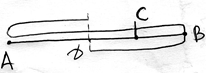
\includegraphics[scale=0.7]{./img/ABC}
\end{minipage}
\end{figure}
\section{Переход на третий  уровень}

В этой теме переход на третий уровень необычен. Проверочная работа включает в себя не только задачи на тему четности и разбиения на пары, но упражнения на умение видеть аналогии.

Если в группе почти все собираются писать проверочную работу для перехода со 2 уровня на 3, то можно сначала первую часть листка разобрать вместе. Иначе -- отвести больше времени на выполнение работы.

Разберем сначала несколько примеров.

\begin{enumerate}
	\item  Двое играют в следующую игру: первый игрок рисует на клетчатой бумаге квадрат. Затем второй игрок зачеркивает одну из клеток этого квадрата. Потом то же делает первый, и так далее. Проигрывает тот, кто не сможет сделать ход. Кто выиграет при правильной игре и как ему надо играть?
	
	\item  Фрекен Бок и Карлсон играют в фантики. Сначала Карлсон вынимает из кармана несколько фантиков, затем фрекен Бок забирает себе один, затем Карлсон и так далее, пока фантики не кончатся. Проигрывает тот, кто не сможет сделать ход. Кто выиграет при правильной игре и как ему надо играть?
\end{enumerate}

Установление аналогии. Пусть в задаче а) первый не рисует квадрат, а выкладывает фантики в виде квадрата, тогда понятно, что в этом случае «забирание» фантика соответствует зачеркиванию клетки квадрата. Тем самым мы показали, что задачи аналогичны.

\begin{enumerate}
	\item  На прямой отметили несколько точек. После этого между каждыми двумя соседними точками отметили еще по точке. Такое "уплотнение" повторили еще дважды (всего три раза). В результате на прямой оказалось отмечено 4009 точек. Сколько точек было отмечено первоначально?
	
	\item  На квартиры была очередь, и около строящегося дома появился очень странный палаточный городок: все палатки были выстроены в линию. Через некоторое время между каждыми двумя поставили ещё по одной палатке. Через некоторое время -- между каждыми двумя снова по одной. Наконец дом достроили. В нём оказалось 15 этажей, на каждом этаже было 3 квартиры. Каждой семье досталось ровно по одной, и все квартиры оказались заняты. Сколько семей приехало сначала, если в одной палатке жила одна семья?
	
	\item В буфете после городской олимпиады выстроилась очередь за бутербродами. Бутерброды задерживались, и в каждый промежуток между стоящими успело влезть по человеку. Бутерброды все еще не начали выдавать, и во все промежутки опять влезло по человеку, а потом еще по человеку. Тут наконец принесли 4009 бутербродов, и всем стоящим досталось по одному. Сколько человек стояли в очереди первоначально?
\end{enumerate}

Установление аналогии. Заметим, что задачи 1 и 3 полностью аналогичны даже численно. Заменим в задаче 3 людей точками, тогда количество принесенных бутербродов в точности совпадает с окончательным количеством людей в очереди, и мы получим формулировку задачи 1. В задаче 2 общее количество семей закамуфлировано под количество квартир, которое надо сначала вычислить. Сделав это, а также заменив семьи (палатки) точками, мы получим задачу 1 с другими численными данными, в которой «уплотнение» произведено только два, а не три раза.

\begin{enumerate}
	\item  Имеется две кучки 9 камней и 10 камней. За один ход можно взять сколько угодно камней из любой (но только одной) кучки. Проигрывает тот, кто не сможет сделать ход. Кто выигрывает при правильной игре?
	
	\item На шахматной доске размером $ 10\times11 $ в левом нижнем углу стоит ладья. Двое по очереди ходят ею вверх или право (влево и вниз ходить не разрешается). Выигрывает тот, кто первым поставит ладью в правый верхний угол. Кто выигрывает при правильной игре?
\end{enumerate}

Установление аналогии. В этом примере аналогия гораздо менее очевидна, однако она есть. Занумеруем вертикали доски от 0 до 10 (слева направо), а горизонтали от 0 до 9 (снизу вверх). Будем устанавливать соответствие следующим образом: представим себе, что мы играем в обе игры одновременно. Будем двигать ладью вверх, если берут камни из кучки с 9 камнями (назовем эту кучку -- первая) и вправо, если из кучки из 10-ю камнями (назовем эту кучку -- вторая). И, наоборот, при движении ладьи по горизонтали будем брать камни из второй кучки, а при движении по вертикали -- из первой. Каждый раз количество взятых камней равно количеству клеток, на которые переместили ладью. Тем самым мы установили соответствие между позициями двух этих игр.\footnote{ Другими словами: мы задаем координаты ладьи на доске и устанавливаем соответствие позиций следующим образом: позиции ладьи ($  a  $ ; $ b  $) соответствует позиция $  a  $ камней в первой кучке и $  b  $ камней во второй.} 

\head{Сентябрь}{Листок 1.2. Четность. Переводная работа. Аналогии.}
\textit{Как узнать, кто вы -- физик или математик? Предлагается решить простейшую задачу: вскипятить воду, если дано: газовая плита, кран с водой, спички. В этом случае действия физика и математика полностью совпадают. Другая задача: вскипятить воду, если дано: все то же самое, но чайник с водой и газ включен. Что сделает физик? Просто поставит чайник на огонь. Что сделает математик? Выключит газ и выльет воду из чайника, чтобы свести задачу к предыдущей, уже решенной!}	
\begin{flushright}
	Из сборника "Физики шутят."
\end{flushright}
\textbf{Найдите аналогичные между собой и аналогичные задачам из листков 1 и 2 уровня. Обращаем внимание, что числа не обязательно совпадают. Обязательно установите аналогию, как это сделано на примерах. Решать все задачи \underline{не нужно}.}
\begin{enumerate}
	\item На 20 кустах малины, растущих в ряд, количество ягод на любых двух соседних кустах отличается на 1. Можно ли собрать с них 2019 ягод? (Оставлять ягоды на кустах нельзя, они сгниют)
	
	\item У фальшивомонетчиков Гоги и Сереги есть 2018 монет номиналом от 1 до 2018 центов. Они хотят так поделить монеты, чтобы номинальная сумма центов у обоих была одинакова. Удастся ли им это сделать?
	
	\item Воевода и его богатыри питаются золотыми рыбками. Воевода наловил 20 золотых рыбок. Тридцать три богатыря передают друг другу чашу с рыбками, и каждый кладет или забирает из чаши рыбку. Может ли в чаше в результате получиться 10 золотых рыбок?
	
	\item У Лизы в 17 спичечных коробках живут 2010 тараканов. На каждом коробке написано количество проживающих в нем тараканов. Может ли произведение этих чисел быть нечетным числом? Если да, то приведите пример, если нет, то докажите, почему.
	
	\item Может ли окружность пересекать в одной точке (без касания!) все стороны правильного 17-ти угольника?
	
	\item У Ильи есть 2018 стальных шариков весом от 1г до 2018г. Он пытается разложить их на две чашки весов так, чтобы весы оказались в равновесии. Сможет ли он это сделать?
	
	\item Катя вернулась из летнего лагеря и заявила, что в лагере, кроме нее, было еще ровно 2018 ребят, и в начале смены каждый был знаком ровно с тремя. Права ли Катя?
	
	\item Куча семиклассников встали в круг, и каждый из них загадал число. После чего Илья Владимирович прошел круг, и для каждых двух соседей подсчитал произведение их чисел. Если у него получалось отрицательное число, то он ставил обоим этим ребятам по двойке. Всего было поставлено 10 двоек. Докажите, что кто-то из семиклассников загадал ноль. 
	
	\item Злой волшебник пообещал Мефодию Буслаеву власть над миром, если он согнет из волшебной золотой проволоки 2019-тиугольник, длины всех сторон которого составляют нечетное число сантиметров. Волшебник дал ему моток такой проволоки длиной 20 м 8 см и сказал, что проволока обязательно должна быть использована полностью. Сможет ли Мефодий получить власть над миром?
	
	\item Кузнечик прыгает по прямой, причем в первый раз он прыгнул на 1см в какую-то сторону, во второй раз -- на 2см, в третий -- на 3см, и так далее. Докажите, что он не сможет за 2018 прыжков вернуться в начальную точку.
	
	\textbf{Запишите решение задачи  8}
	
\end{enumerate}

Еще раз обращаем внимание, что в данной работе не требуется приводить решения всех задач. Для успешной сдали нужно указать аналогии и записать решение лишь одной задачи.

\section{Решения проверочной работы с уровня 2 на уровень 3}
%
% Тут нужно привести аналогии и решение задачи 1.8
%

Задачи 2 и 6 полностью аналогичны таким образом: монеты -- гири. В обоих задачах требуется разделить их пополам. Также они схожи с задачей 10, в которой прыжок вправо -- монета одному фальшивомонетчику, а прыжок влево - другому. Условие совпадения суммы денег эквивалентно условию попадания в начало координат.
Задача \ref{1.16} аналогична этим трем - 2, 6, 10.

%После урока математики Вася вышел из школы и решил двигаться вдоль проспекта. Сначала он переместился на 1 шаг в какую-то сторону, затем на два шага, потом на 3 и т.д. Сможет ли Вася, сделав в очередной раз 2019 шагов, вернуться в начальную точку?
%
%\begin{prf}	
%	\textbf{1 способ.} Назовем направление вправо положительным, а направление влево – отрицательным. Пусть точка, из которой Вася начал движение, будет начальной. Будем определять в шагах расстояние от начальной точки следующим образом: если Вася идет вправо на какое-то количество шагов n, то будем прибавлять n к уже имеющейся сумме, и вычитать, если он идет влево на n шагов, то вычитать. Таким образом, задача свелась к возможности расставить «плюсы» и «минусы» перед числами от 1 до 2019 так, чтобы в сумме получился ноль. Посмотрим, какие числа вообще могут получаться. Поскольку, среди 2019 последовательных чисел -- 1010 нечетных и 1009 четных, то знакопеременная сумма в любом случае будет нечетной. Следовательно, ноль получить не удастся, так как ноль – число четное.
%	
%	\textbf{2 способ.} Предположим, Васе удалось вернуться в исходную точку. Тогда сумма шагов вправо равна сумме шагов влево. Но тогда сумма всех шагов должна быть четной. Но это не так, поскольку сумма всех натуральных чисел от 1 до 2017 нечетна.
%\end{prf}

\begin{table}[h]\centering
	\begin{tabular}{|c|c|}
		\hline
		номер в проверочной&номер в листках 1.1, 1.2\\
		\hline
		1,3&\ref{an3.2},\ref{1.9},\ref{an1.3}\\
		\hline
		4&\ref{an4.1}\\
		\hline
		5&\ref{an5.1}\\
		\hline
		8&\ref{1.10},\ref{1.11}\\
		\hline
		9&\ref{1.15}\\
		\hline
	\end{tabular}
\end{table}
\begin{prf}
	Задачи 8. Предположим противное, что 0 никто не загадал. Тогда пар соседей, у которых произведение отрицательно четно. Потому что количество пар <<->> <<+>> ровно столько же, сколько пар <<+>> <<->> (если идти, например, по часовой стрелке). А 10 -- это 5 пар. Противоречие.
\end{prf}

\section{Дубль уровня 2}

Второй уровень достаточно сложен. Поэтому скорее всего дубль этого листка потребуется.
\head{Октябрь}{Листок 1. Четность. Уровень 2А}



\begin{thm}
	\label{f1}
	На рисунке прямая пересекает все стороны шестиугольника. Может ли прямая пересекать все стороны какого-нибудь 17-угольника, не проходя ни через одну его вершину?
\end{thm}

%\begin{prf}
%	Заметим, что прямая делит плоскость на две полуплоскости. Отрезок пересекается с такой прямой тогда и только тогда, когда концы отрезка лежат по разные стороны от прямой, то есть в различных полуплоскостях. Поэтому если мы начнем обход многоугольника по часовой стрелке, при переходе к следующей вершине будем менять полуплоскость, в которой находимся. Но тогда первая и семнадцатая вершины окажутся в одной полуплоскости, а значит, отрезок, их соединяющий, не будет пересекаться с прямой. Противоречие.
%\end{prf}

\begin{thm}
	По кругу зацеплены 17 шестерёнок: первая со второй, вторая с третьей \dots семнадцатая с первой. Могут ли они вращаться?
\end{thm}

\begin{thm}100 фишек поставлены в ряд. Разрешено менять местами любые две фишки, стоящие через одну. Можно ли поставить фишки в обратном порядке?
\end{thm}

\begin{thm}
	Кузнечик прыгает по прямой, причем в первый раз он прыгнул на 1см в какую-то сторону, во второй раз – на 3см, в третий – на 5см, и так далее. Сможет ли он за 2011 прыжков вернуться в начальную точку?
\end{thm}

\begin{thm}
	В 7Ю учится 30 человек. На каждый день нужно назначить трое дежурных. Можно ли так составить график дежурства, чтобы через некоторое время каждый подежурил с каждым ровно один раз?
\end{thm}

\begin{thm}
	На шахматной доске стоят 17 шашек, расположенных симметрично относительно большой диагонали. Докажите, что есть шашка или шашки и на большой диагонали.
\end{thm}	

\begin{thm}
	Витя и Коля купили несколько шоколадок «Вдохновение»\footnote{Шоколадка «Вдохновение» состоит из нескольких отдельных плиток, каждая из которых содержит две дольки.} и решили их поделить между собой. Каждую плитку брал себе целиком либо Витя, либо Коля, либо они ломали ее пополам. После этого Витя заявил, что Коля взял себе на одну дольку больше. Могло ли такое быть? 
\end{thm}
\begin{figure}[h]\centering
	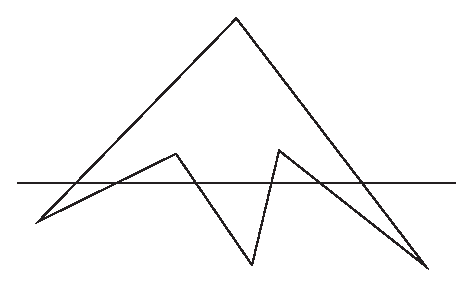
\includegraphics[width=8 cm]{./img/six}
	\caption{\textbf{Задача \ref{f1}}}
\end{figure}

\head{Октябрь}{Листок 1. Четность. Переводная работа 2А. Аналогии.}

\textbf{Найдите аналогичные между собой и аналогичные задачам из листков 1 и 2 уровня. Обращаем внимание, что числа не обязательно совпадают. Обязательно установите аналогию, как это сделано на примерах.}

\textbf{Задача 1A.} У двоечника Вани есть 2019 дневников. Он хочет разложить их по кругу так, чтобы количество двоек в лежащих рядом дневниках отличалось на 1. Сможет ли он это сделать?

\textbf{Задача 2A.} На далекой планете Занзибар живут многоножки. Как-то собрались вместе 2018 многоножек с количеством ножек от 1 до 2018. Причем известно, что у всех количество ножек разное. Они хотят разбиться на две команды для игры в крокет, чтобы общее количество ножек в командах было одинаково. Удастся ли им это сделать?

\textbf{Задача 3A.} Михаил Владимирович написал на доске программу, содержащую 2019 строчек. После чего каждый из 20 учеников 7Ю класса вышел к доске (один или несколько раз) и дописал или стер одну строчку программы. В результате на доске оказалась записанной программа из 17 строчек. Докажите, что нечетное число раз к доске выходило четное число учеников.

\textbf{Задача 4A.} У Жени в 20 аквариумах живут 2019 креветок. На каждом аквариуме написано количество проживающих в нем креветок. Может ли произведение этих чисел быть нечетным числом? Если да, то приведите пример, если нет, то докажите, почему.

\textbf{Задача 5A.} Шахматный конь обошел все клетки шахматной доски 7х7. Мог ли он начать не с угловой клетки, а с соседней с угловой?

\textbf{Задача 6A.} У Ильи есть 2018 стальных шариков весом от 1г до 2018г. Он пытается разложить их на две чашки весов так, чтобы весы оказались в равновесии. Сможет ли он это сделать?

\textbf{Задача 7A.} Незнайка, вернувшись из путешествия, рассказывал, что в некоторой планетарной системе 2019 планет, причем каждая имеет межпланетное сообщение еще с тремя другими. Не заблуждается ли Незнайка?

\textbf{Задача 8A.} Лизочка играет в Зазеркалье. Каждый день она меняем имя. Если она сегодня звалась Лиза, то на следующий день -- Лизавета. Если же сегодня она звалась Лизавета, то на следующий день она зовется Лизой. А еще она меняет цвет платья -- два дня носит красное, а потом два дня -- синее. 1 сентября она назвалась Лизой и пришла в белом, а на следующий день уже надела красное. В каком платье и с каким именем она встретит Новый Год?\footnote{31 декабря} 

\textbf{Задача 9A.} Злой волшебник пообещал Мефодию Буслаеву власть над миром, если он соберет волшебные бусы из 49 камней, чередуя алмаз и бриллиант. Причем, чтобы алмазов было меньше, чем бриллиантов, а начинались бусы с алмаза. Сможет ли Мефодий получить власть над миром?

\textbf{Задача 10A.} Кузнечик прыгает по прямой, причем в первый раз он прыгнул на 1см в какую-то сторону, во второй раз -- на 2 см, в третий -- на 3 см, и так далее. Докажите, что он не сможет за 2010 прыжков вернуться в начальную точку.

\textbf{Задача 11A.} Докажите, что число способов расставить на шахматной доске $ 2018\times2018 $ 2018 ферзей так, чтобы они не били друг друга, четно.

\textbf{Запишите решения задач  8  и  3}
\hrule

\section{ Уровень третий}

Как показывает практика, до третьего уровня добираются далеко не все. Задания этого уровня достаточно сложны и требуют от школьников уже не только владения материалом, но и значительной доли фантазии и сообразительности. 
\head{Cентябрь}{Листок 1. Четность. Уровень 3.}

В этом разделе собраны задачи, для решения которых придется применить несколько идей, разобранных в листках уровней 1 и 2.
\begin{thm}
	Лёша нарисовал на клетчатой бумаге замкнутый путь, идущий по линиям сетки. Докажите, что он нарисовал четное число единичных отрезков (единица -- сторона клетки).
\end{thm}
\begin{thm}\label{1.23}
	Улитка ползет по плоскости с постоянной скоростью. Каждые 15 минут она поворачивает под прямым углом. Докажите, что вернуться в исходную точку она сможет только через целое число часов.
\end{thm}
\begin{thm}
	Кузнечик прыгает а) по прямой на  метр вправо или влево; б) по плоскости, каждым прыжком перемещаясь на метр на север, юг, запад или восток; в)  по узлам клетчатой плоскости, каждым прыжком перемещаясь по диагонали одной из клеток. Может ли он вернуться в исходную точку через 2011 прыжков?
\end{thm}
\begin{thm} а) б) в)
	Может ли в условиях предыдущей задачи кузнечик вернуться в исходную точку через 2010 прыжков?
\end{thm}
\begin{thm}
	${}^{n}$ Дорожки парка -- линии квадратной сетки. Одна ячейка -- 100 на 100 метров. Войти в парк можно через единственный вход, а выйти -- через единственный выход. Петя и Вася делились впечатлениями по поводу прогулок и выяснили, что один прошел по дорожкам на 300 м меньше, чем другой, причем каждый обошел целое число дорожек (то есть, ступив на дорожку, проходил до конца без возвращений). Не ошиблись ли ребята?
\end{thm}
\begin{thm}\label{1.27}
	К 17-значному числу прибавили число, записанное теми же цифрами, но в обратном порядке. Докажите, что хотя бы одна из цифр полученной суммы четна.
\end{thm}
\begin{thm}
	17 девочек и 17 мальчиков встали в хоровод. Докажите, что у кого-то с обеих сторон стоят девочки.
\end{thm}
\begin{thm}
	Маша и ее друзья встали в круг. Оказалось, что у каждого из них оба соседа либо оба мальчики, либо девочки. Мальчиков среди Машиных друзей пять. А сколько девочек?
\end{thm}
\begin{thm}
	Во время перемирия за круглым столом разместились рыцари двух враждующих станов. Оказалось, что число рыцарей, справа от которых сидит враг, равно числу рыцарей, справа от которых сидит друг. Докажите, что число рыцарей делится на 4.
\end{thm}
\begin{thm}\label{1.31}
	В классе 30 учеников. Они сидят за 15-ю партами. При этом оказалось, что ровно половина всех девочек сидит с мальчиками. Докажите, что их не удастся пересадить (за те же 15 парт) так, чтобы ровно половина всех мальчиков класса сидела с девочками.
\end{thm}
\begin{thm}\label{1.32}
	Сто грустных мартышек кидают друг в друга одним кокосовым орехом. Грустная мартышка, попавшая орехом в другую грустную мартышку, становится веселой и больше не грустнеет. Мартышка, в которую попали, выбывает из игры. Каких мартышек больше выбыло из игры -- веселых или грустных -- к моменту, когда в игре осталась одна мартышка?
\end{thm}
\newpage
\section{Подведение итогов  и результаты.}

 Итак, подошло время подведения итогов. Поскольку это первый листок и школьники привыкают к новым правилам, к самостоятельной работе, то время, которое обычно отводится на листок -- около полутора месяцев -- примерно 12 полуторачасовых занятий. Детям заранее объявляется, когда наступает «час Х», то есть день, когда задачи будут разобраны и их решения больше принимать не будут. Лучше не устраивать разбор всех задач в самом конце, а разбирать их по ходу дела. И школьникам будет проще воспринимать, и пользы от этого больше. Например, задачи листка 1 уровня рекомендуется разобрать, когда все уже готовы писать (или уже написали) проверочную работу на 1 уровень. Часть задач второго уровня можно разбирать в процессе, когда есть такая необходимость. Если в этом случае задача рассказывается тому, кто ее не смог решить, то задачу можно заменить на похожую. Главная цель -- убедиться, что все ученики класса разобрались в решении всех задач 1 и 2 уровня.

 В уровне 3 некоторые задачи могут остаться неразобранные, если нет людей, кто над ними думал. С другой стороны, если школьники выражают желание узнать решения задач, стоит им их рассказать. 

 Мы считаем, что обязательному разбору подлежат задачи из листка 3 уровня -- \ref{1.23}, \ref{1.27}, \ref{1.31} и \ref{1.32}

 Оценки. Если эти листки решаются в школе, а не на кружке, то по правилам школы необходимым является выставление оценок. 

 Школьники, сдавшие листок 1 уровня и написавшие переводную работу на 2 уровень, но далее не продвинувшиеся, получают оценку «3» или «удовлетворительно».

 Школьники, сдавшие листок 2 уровня и написавшие переводную работу на 3 уровень, но далее не продвинувшиеся, получают оценку «4» или «хорошо».

 Школьники, сдавшие листок 2 уровня и написавшие переводную работу на 3 уровень и решившие не менее 8 задач из листка уровня 3, получают оценку «5» или «отлично». 

 Дополнительную оценку «5» можно поставить тем, кто решил все задачи листка уровня 3.

 При этом не имеет значения решил школьник задачи проверочной работы с первого или со второго раза.


\section{ Решения некоторых задач.}

\textbf{Задача \ref{1.10}}
Полный комплект костей домино выложен в цепочку. На одном конце оказалась пятерка. А что могло оказаться на другом?


\begin{prf}
	Рассмотрим множество половинок всех доминошек. Всего доминошек 28, при этом каждое число (от 0 до 6) присутствует ровно на 8 половинках. Заметим, что в выложенной цепочке все половинки кроме двух крайних разбиты на пары с одинаковыми цифрами. Это означает, что среди них любое число (от 0 до 6) встречается четное число раз. Тогда, если не рассматривать неизвестный конец, пятерка встречается на одном конце и еще на четном количестве мест, а все остальные числа встречаются на четном количестве мест. Отсюда однозначно следует, что на втором конце тоже пятерка.
\end{prf}

\textbf{Задача \ref{1.11}}
Из полного набора домино, подаренного родителями, Ваня потерял все кости с «пустышками». Сможет ли теперь кто-нибудь выложить оставшиеся кости в ряд?

\begin{prf}
	Не сможет. Предположим обратное: пусть кости разложены в ряд. Все половинки, кроме двух крайних, объединяются в пары с равными числами. На двух крайних числа могут быть как равные, так и нет (мы не можем ссылаться в этом месте на предыдущую задачу, так как часть косточек потеряна). Следовательно, все числа, за исключением двух, заведомо появляются четное число раз. Но после потери всех пустышек осталось ровно по 7 экземпляров каждой из 6 цифр 1,2,3,4,5,6. 
\end{prf}



\textbf{Задача \ref{1.23}}
Улитка ползет по плоскости с постоянной скоростью. Каждые 15 минут она поворачивает под прямым углом. Докажите, что вернуться в исходную точку она сможет только через целое число часов.
\begin{prf}
	Введем координаты. Оси направим параллельно и перпендикулярно движению улитки. А нулем обозначим ее начальное положение. Пусть за 15 минут улитка проползает 1. Тогда: \\за 15 минут улитка меняет четность одной координаты.\\ за 30 минут улитка меняет четность каждой координаты\\ за 45 минут четность хотя бы одной координаты останется измененной\\ за час четность каждой координаты не изменится\\
	Потому что изменение координаты чередуется каждые 15 минут. Значит за нецелое количество часов вернуться назад (то есть не менять четность), нельзя.
\end{prf}

\textbf{Задача \ref{1.27}}
К 17-значному числу прибавили число, записанное теми же цифрами, но в обратном порядке. Докажите, что хотя бы одна из цифр полученной суммы четна.
\begin{prf}
	Предположим противное. Посмотрим на 9 цифру: она складывается сама с собой, поэтому у суммы в 9 разряде будет четное, если нет перехода с 8 разряда. Значит есть и переход с 10 на 11 разряд (потому что участвуют те же цифры). Следовательно четность 11 и 7 цифр одинакова. \\ Поэтому у суммы в 7 разряде будет четное, если нет перехода с 6 разряда. Значит есть и переход с 6 на 7 разряд (потому что участвуют те же цифры). Следовательно четность 12 и 6 цифр одинакова.
	\\ повторяя аналогичные рассуждения приходим к тому, что четность 17 и 1 цифр одинакова.
	Но на 1 и 17 местах цифры разной четности (иначе последняя цифра суммы была бы четной). Противоречие.
\end{prf}

\textbf{Задача \ref{1.31}}
	В классе 30 учеников. Они сидят за 15-ю партами. При этом оказалось, что ровно половина всех девочек сидит с мальчиками. Докажите, что их не удастся пересадить (за те же 15 парт) так, чтобы ровно половина всех мальчиков класса сидела с девочками.
\begin{prf}
	Если половина всех девочек сидит с мальчиками, то остальная сидит с девочками, то есть по парам. Значит число девочек делится на 4. Для аналогичного условия для мальчиков требуется делимость их количества на 4. Но тогда сумма всех детей должна делиться на 4. Но 30 не делится на 4. Противоречие.
\end{prf}

\textbf{Задача \ref{1.32}}
	Сто грустных мартышек кидают друг в друга одним кокосовым орехом. Грустная мартышка, попавшая орехом в другую грустную мартышку, становится веселой и больше не грустнеет. Мартышка, в которую попали, выбывает из игры. Каких мартышек больше выбыло из игры -- веселых или грустных -- к моменту, когда в игре осталась одна мартышка?
\begin{prf}
	Веселых меньше. Чтобы попасть в веселую, она перед этим должны была попасть в грустную. Значит веселых, в которых попали, меньше или равно количеству выбитых грустных. Равенства быть не может в силу нечетности количества выбитых.
\end{prf}
% 2 уровня 12, 14, 15, 16

\textbf{Задача \ref{1.12}}
	На бирже в городе Нью-Васюки ежедневно в 10.00 проходят торги. Рано утром 1 января N-го года цены на акции фирм «Вася Inc.» и «Петя и Ко» были один и два рубля соответственно. Вечером 31 декабря того же года цены стали снова теми же. Лёша установил, что цены на акции этих фирм всегда были различны, каждый день изменялись и все время были либо один, либо два рубля. Докажите, что прошедший год был високосным.

\begin{prf}
	Каждый день четность стоимостей акций меняется. Значит такой же стоимость может стать только через четное количество дней. Только в високосном году так бывает.
\end{prf}

\textbf{Задача \ref{1.14}} Можно ли выписать в ряд по одному разу цифры от 1 до 9 так, чтобы между единицей и двойкой, двойкой и тройкой, \dots, восьмеркой и девяткой было нечетное число цифр?

\begin{prf}
	Предположим, что у нас получилось их выписать в таком порядке. Тогда единица и двойка стоят на местах одинаковой четности. Ровно как и любые другие 2 соседних по величине числа. Значит все числа стоят либо на четных, либо на нечетных местах, чего быть, конечно, не может.
\end{prf}


\textbf{Задача \ref{1.15}} 7М класс упражняется в счете. Анатолий Анатольевич написал на доске число 2011. После чего каждый ученик вышел к доске, прибавил или вычел 17 или 13 и записал получившийся результат. Когда каждый из 20 учеников вышел по одному разу, на доске оказалось написано число 2012. Анатолий Анатольевич посмотрел на доску и расстроился. Докажите, что кто-то из учеников ошибся.

\begin{prf}
	Каждая операция меняет четность числа. Через 20 операция четность не должна измениться, значит кто-то ошибся.
\end{prf}


\textbf{Задача \ref{1.16}}
	У Вини-Пуха было 2019 горшочков меда. Кристофер Робин принес или забрал 9 горшочков, что именно – Пух не помнит. На следующий день Кристофер Робин снова пришел и принес или забрал 8 горшочков, на следующий день – 7 и так далее. Наконец Кристофер Робин пришел и принес или забрал один горшочек.  а) Могло ли у Винни-Пуха на 10 день оказаться горшочков столько же, сколько и было в самом начале, то есть 2019? б) Сколько вообще горшочков меда могло быть у Вини-Пуха на 10 день, если все это время он мед не ел?

\begin{prf}
	а) за 10 дней четность количества горшочков менялась 5 раз, значит в конце должно было получиться четное количество, значит 2019 быть не могло.\\
	б) можно получить любую четную сумму от $2011-45=1966$ до $2019+45=2056$. Доказательство опустим. 
%	Пусть получена сумма $ n $, докажем, что можно получить $n+2$, если $ n $ не равно 2056. Если в последний день горшок был <<забран>> -- <<->>, то изменив забор на <<приношение>> -- <<+>> можно получить искомую сумму. В противном случае посмотрим на предыдущий день, когда Робин взял или отдал 2 горшка. 
\end{prf}

% 1 уровня -- 7, 8, 10
%
\textbf{Задача \ref{1.7}}
	На доске написано 2019 целых чисел. Всегда ли можно стереть одно из них так, чтобы сумма всех оставшихся чисел была четна?

\begin{prf}
	Да, если сумма четна, то среди чисел есть хотя бы одно четное, которое можно зачеркнуть. В противном случае есть хотя бы одно нечетное, которое тоже можно зачеркнуть.
\end{prf}


\textbf{Задача \ref{1.9}}
	Вокруг круглой поляны растут 2019 сосен. Незнайка измерил высоту каждой из них и заявил, что любые две соседние сосны отличаются по высоте ровно на метр. Знайка тут же заметил, что Незнайка врет. Кому верить?
\begin{prf}
	Высота всех деревьев, стоящих на нечетных местах одинакова. Но 1 и 2019 сосны стоят рядом, и их высоты не могут отличаться на 1. Значит Незнайка врет.
\end{prf}

\chapter{Принцип Дирихле}
\head{Октябрь}{Теоретический Листок. Принцип Дирихле}
\epigraph{\textit{Если у тебя в двух карманах три копейки, то в одном из них меньше 2 копеек.}}{Народная мудрость}

При решении самых различных задач часто бывает полезен так называемый «принцип Дирихле», названный в честь немецкого математика Петера Густава Лежена Дирихле (1805 – 1859); по-другому этот принцип еще называют «принципом ящиков» или «принципом голубятни» . Этот принцип часто является хорошим средством при доказательстве важнейших теорем  в теории чисел, алгебре, геометрии. Возможно, вы уже слышали про этот принцип. И скорее всего, в первый раз вы услышали его формулировку в таком шутливом виде: "Пусть есть n клеток, в которых сидят не менее $n+1$ кроликов. Тогда найдется клетка, в которой сидит не меньше двух кроликов." Доказательство этого факта чрезвычайно просто. Предположим, что это не так. Т.е. в каждой клетке сидит не более одного кролика (один или ни одного). Тогда, так как клеток n, то в клетках сидит не более, чем n кроликов, что противоречит условию. Обратите внимание, что мы не можем указать, в какой именно клетке сидит больше одного кролика (даже не можем сказать, \textbf{НА} сколько больше), мы можем только утверждать, что такая клетка обязательно есть. Полученных сведений совсем мало, однако, и на основании таких, казалось бы, незначительных сведений можно делать значительные выводы.
Разберем на примерах:
\begin{thm}
	В коробке лежат шарики двух цветов. Сколько шариков достаточно наугад вынуть из коробки, чтобы среди них заведомо нашлись два одного цвета? 
\end{thm}

\begin{prf}
	Понятно, что двух шариков недостаточно. Может оказаться один черный, другой белый. Вынем три шарика. Т.к. цвета всего два, то, очевидно, что два шарика будут одного цвета. Т.е. достаточно вынуть три шарика.\footnote{Вытаскивая три шарика, мы будем уверены, что сможем выбрать из них два одного цвета, но НЕ ЗНАЕМ, КАКОГО! – черного или белого.}
\end{prf}

\begin{thm}
	В лесу растет миллион ёлок. Известно, что на каждой из них не более 400 000 иголок. Докажите, что в лесу найдутся по крайней мере три ёлки с одинаковым числом иголок.
\end{thm}

\begin{prf}
	Будем рассаживать наших «кроликов–ёлок» по «клеткам» с номерами от 0 до 400 000. В одну «клетку» будем «сажать» те ёлки, у которых число иголок равно номеру клетки. Задача будет решена, если мы докажем, что найдет «клетка», в которой «сидит» не менее трех ёлок. Всего «клеток» 400 001 штука. И если бы в каждой из них сидело не более двух «кроликов – ёлок», то всего ёлок было бы не более, чем  $2\times400001=800002$ штук. А это не так. Следовательно, найдется хотя бы одна «клетка» в которой не менее 3 «кроликов». \footnote{Мы доказали, что таких елок не менее трех, но мы не знаем точно, сколько их. Может быть, 5, может быть, 100, а может быть и весь миллион. Более того, мы не знаем, сколько конкретно, иголок на них. Может, 5, может, 400 000, а может и ни одной!}
\end{prf}

Иногда принцип рассуждений, использованный в предыдущей задаче, еще называют \textit{обобщенным принципом Дирихле}: \textit{Если в N клетках сидит не менее $(k\times N)+1$ кролик, то найдется клетка, в которой сидит не менее $k+1$ кролика.}

Заметим, что при $k =1$ обобщенный принцип Дирихле превращается в обычный принцип Дирихле.

\begin{ex}\label{u12}
	Закончите предложения:\\
	а) В пяти тарелках лежат шесть конфет. Тогда найдется тарелка, в которой лежит \dots\\
	б) В 17 чуланах живут 19 привидений. Значит найдется чулан, в котором живет \dots\\
	в) В 10 спичечных коробках лежит 21 монетка. Тогда найдется коробок, в котором лежит \dots	
\end{ex}

\begin{ex}\label{u13}	25 голубей рассадили по 7 клеткам. Укажите, какие из приведенных ниже утверждений всегда верны: \\
	а) «найдется клетка, в которой 4 голубя»;     б) «найдется клетка, в которой не менее 4 голубей»;
	в) «найдется клетка, в которой больше 4 голубей»; г) «найдется клетка, в которой 3 голубя»;\\
	д) «найдется клетка, в которой меньше 3 голубей»; е) «найдется клетка, в которой не более 3 голубей».
\end{ex}
\head{Октябрь}{Листок 1. Принцип Дирихле}
\epigraph{\textit{Если ты в своем кармане ни копейки не нашел, загляни в карман к соседу – очевидно, деньги там!}}{Григорий Остер "Вредные советы"}
\begin{thm}$^\circ$
	В ящике лежат шары: 5 красных, 7 синих и 1 зеленый. Сколько шаров надо вынуть, не глядя, чтобы наверняка достать 2 шара одного цвета?
\end{thm}

\begin{thm}
	На Марс привезли 51 ящик с приборами пяти видов. Верно ли, что обязательно приборов какого-то вида было а) не более 10 ящиков, б) не менее 10 ящиков?
\end{thm}

\begin{thm}\label{2.3}
	$^n$ Вася в течение 3 дней съел 100 шоколадок. Обязательно ли найдется ли день, в который Вася съел а) не менее 34 шоколадок б) не более 33 шоколадок?
\end{thm}

%\begin{prf}
%	а) Предположим противное: такого дня не найдется. Это означает, что в каждый из трех дней Вася съедал менее 34 шоколадок, то есть 33 или менее. Тогда за три дня он мог съесть максимум $3\times33=99$ шоколадок, а он съел больше -- 100. Противоречие. Следовательно, наше предположение неверно и такой день найдется.
%	
%	б) Предположим противное: такого дня не найдется. Это означает, что в каждый из трех дней Вася съедал более 33 шоколадок, то есть 34 или более. Тогда за три дня он мог съесть минимум $3\times34=102$ шоколадок, а он съел меньше -- 100. Противоречие. Следовательно, наше предположение неверно и такой день найдется.
%\end{prf}

\begin{thm}
	а) В темной комнате стоит шкаф, в ящике которого лежат 24 черных и 24 синих носка. Сколько носков следует взять из шкафа, чтобы из них заведомо можно было составить по крайней мере одну пару носков одного цвета? (речь идет о минимальном числе носок)	
	б) Сколько надо взять носков, чтобы заведомо можно было составить хотя бы одну пару носков черного цвета?	
	в) Как изменится решение задачи, если в ящике лежат 12 пар черных и 12 пар синих ботинок и требуется составить пару одного цвета (как в пункте а) и пару черного цвета (как в пункте б)?
\end{thm}

\begin{thm}
	Белых и черных кроликов рассаживали по клеткам. Белых было больше, чем черных. Докажите, что найдется клетка, в которой белых кроликов больше, чем черных.
\end{thm}

\begin{thm}
	В коробке лежат карандаши: 7 красных и 5 синих. В темноте берут карандаши. Сколько надо взять карандашей, чтобы среди них было не меньше 2-х красных и не меньше 3-х синих? 
\end{thm}

\begin{thm}
	В ящике лежат цветные карандаши: 10 красных, 8 синих и 4 желтых. В темноте берем из ящика карандаши. Какое наименьшее число карандашей надо взять, чтобы среди них заведомо было:\\
	а) не менее 4-х карандашей одного цвета?~~
	б) не менее 6-ти карандашей одного цвета?\\
	в) хотя бы 1 карандаш каждого цвета?~~~~~~
	г) не менее 6-ти синих карандашей? 
\end{thm}

\begin{thm}
	Докажите, что среди любых $n$ чисел найдутся два, разность\footnote{Здесь вам понадобится понятие остатка при делении целых чисел.} которых делится на $n-1$. 
\end{thm}

\begin{thm}
	В классе 40 человек. В диктанте Степа сделал 13 ошибок, а остальные сделали меньше. Обязательно ли найдутся ли среди них а) 3 человека, б) 4 человека, сделавших одинаковое число ошибок?
\end{thm}

\begin{thm}
	У человека на голове не более $400000$ волос, в Москве более 8 млн. жителей. Докажите, что найдутся 20 москвичей с одинаковым числом волос.
\end{thm}

\begin{thm}
	О населении города Поданк известно следующее:\\
	а) Среди жителей Поданка не найдется двух с равным числом волос на голове.\\
	б) Ни у одного жителя Поданка не голове не растет ровно 518 волос.\\
	в) Жителей в Поданке больше, чем волос на голове любого из них.\\
	Какова может быть наибольшая численность населения г. Поданка?
\end{thm}
\textit{Напоминаем, что получения задач следующего уровня необходимо выполнить проверочную работу, включающую задачи, похожие на приведенные выше. Задачи, отмеченные значком п, приниматься в устном форме не будут. В данном случае это единственная задача \ref{2.3}. Решение таких задач надлежит выполнить в письменном виде дома и принести на занятие спецматематики.
	Рекомендуем решать задачи по порядку, поскольку зачастую в решении следующей задачи можно использовать идею из предыдущей.
	\begin{flushright}
		Желаем успеха!
	\end{flushright}
}

\head{Октябрь}{Листок 1. Принцип Дирихле. Проверочная работа.}
\begin{thm}
	Докажите, что среди любых шести человек всегда найдутся либо трое попарно знакомых, либо трое попарно незнакомых.
\end{thm}

\begin{thm}
	Каждый из 17 ученых переписывается с остальными. В их переписке речь идет лишь о трех темах. Каждая пара ученых переписывается друг с другом только по одной теме. Докажите, что не менее трех ученых переписываются друг с другом по одной и той же теме.
\end{thm}

\begin{thm}
	В погребе стоит 20 одинаковых банок с вареньем. В 8-ми банках клубничное варенье, в 7-ми – малиновое, в 5-ти – вишневое. Каково наибольшее число банок, которые можно в темноте вынести из погреба с уверенностью, что там осталось еще хотя бы 4 банки одного сорта варенья и 3 банки другого? 
\end{thm}

\begin{thm}
	За круглым столом сидят 25 детей и 25 преподавателей и грустно смотрят друг на друга.
	а) Докажите, что есть ребенок, который сидит точно напротив преподавателя.
	б) Докажите, что есть несчастный, оба соседа которого – дети.
\end{thm}
\begin{thm}
	$^{\ast\ast}$В классе 25 человек. Известно, что среди любых трех из них есть двое друзей. Докажите, что есть ученик, у которого не менее 12 друзей.
\end{thm}

\head{Октябрь}{Листок 2. Принцип Дирихле.}

\epigraph{ \textit{«В три клетки нельзя посадить четырех зайцев так, чтобы в каждой клетке сидел ровно один заяц. Это следует из принципа Дирихле\dots} \\ \textit{Заменим ученых кроликами и посадим их в ящики\dots}»}{Из школьных записей}
В предыдущих задачах было ясно из условия, что именно надо считать “клетками”, а что – “кроликами”. Обычно угадать “кроликов” несложно. Скорее всего, это те объекты, про которые и надо что-то выяснить, хотя это и не всегда. Иногда надо рассматривать не все предложенные объекты, а только часть из них, или, наоборот, добавить к ним еще несколько и рассматривать все полученное множество. Перед решением каждой из следующих задач мы попросим вас указать, что именно вы считаете «клетками», а что – «кроликами»

\begin{thm}
	Докажите, что равносторонний треугольник нельзя покрыть двумя меньшими равносторонними треугольниками.
\end{thm}

\begin{thm}\label{2.13}
	$^n$ В спичечных коробках находятся 50 тараканов. Докажите, что либо в одном коробке живут 8 тараканов, либо для выкидывания коробков по одному в день потребуется больше недели.
\end{thm}
%
%\begin{prf}
%	Предположим противное: в каждом коробке живут не более 7 тараканов и таких коробков не более семи (поскольку в неделе семь дней). Тогда в этих коробках живет максимум 7х7=49 тараканов, но у нас их больше. Противоречие. Следовательно, наше предположение неверно и либо в одном коробке живут 8 или более тараканов, либо для выкидывания коробков по одному в день потребуется больше недели.
%\end{prf}

\begin{thm}
	По краю круглого стола расставлены таблички с фамилиями дипломатов, участвующих в переговорах о борьбе с мировым терроризмом. Оказалось, что дипломаты не посмотрели на таблички и каждый сел не на свое место. Можно ли повернуть стол так, чтобы хотя бы два дипломата сидели против своих табличек?
\end{thm}

\begin{thm}
	$^\ast$Докажите, что среди чисел, записываемых одними единицами, найдется число, делящееся на 2007.
\end{thm}

\begin{thm}
	$^\ast$Карабас Барабас пообещал Буратино открыть тайну Золотого ключика, если тот составит из чисел 0, 1, 2 волшебный квадрат 6х6 так, что в каждой строке, каждом столбце и двух диагоналях сумма чисел была различна. Помогите Буратино!
\end{thm}

\begin{thm}
	$^\ast$Дано 11 различных натуральных чисел, не превосходящих 20. Докажите, что из них можно выбрать два, одно из которых делится на другое. 
\end{thm}

\begin{thm}
	Докажите, что среди любых трех целых чисел найдется два, сумма которых четна.
\end{thm}

\begin{thm}
	$^{\ast\ast}$ Докажите, что среди любых 10 целых чисел найдутся одно или несколько, сумма которых делится на 10.
\end{thm}

\begin{thm}
	Докажите, что среди любого количества человек найдутся двое, имеющих одинаковое (возможно, нулевое) число знакомых среди этих человек.
\end{thm}

\begin{thm}
	Александр Кириллович предложил ученикам 7Ю класса написать два теста, за каждый из которых можно было получить оценку 1, 2, 3, 4 или 5. Верно ли, что обязательно найдутся два ученика получившие одинаковые оценки по обоим тестам, если в 7Ю учится 26 человек?
\end{thm}

\begin{thm}
	В ковре размером 4х4 метра моль проела 15 дырок. Докажите, что из него можно вырезать коврик размером 1х1 метр, не содержащий внутри себя дырок. (Дырки считайте точечными.)
\end{thm}

\textit{Напоминаем, что получения задач следующего уровня необходимо выполнить проверочную работу, включающую задачи, похожие на приведенные выше. Задачи, отмеченные значком п, приниматься в устном форме не будут. В данном случае это единственная задача \ref{2.13}. Решение таких задач надлежит выполнить в письменном виде дома и принести на занятие спецматематики.
	Рекомендуем решать задачи по порядку, поскольку зачастую в решении следующей задачи можно использовать идею из предыдущей.
	\begin{flushright}
		Желаем успеха!
	\end{flushright}
}

\head{Октябрь}{Листок 2.2. Принцип Дирихле. Проверочная работа. Аналогии.}

И снова аналогии! В это раз в этом разделе нет оригинальных задач. Поэтому решать их вам не придется. Для выполнения этого задания вам нужно только найти задачи, аналогичные приведенным выше и описать соответствие.

\begin{thm}
	В кружок ходит 17 школьников. На дом им задали 3 задачи. Как потом оказалось, каждые два школьника посоветовались друг с другом ровно по одной задаче. Докажите, что найдется три кружковца, посоветовавшиеся попарно друг с другом по одной и той же задаче.
\end{thm}

\begin{thm}
	На бумаге нарисованы шесть точек. Каждые две из них соединены либо красным отрезком, либо синим. Докажите, что найдется либо красный треугольник с вершинами в нарисованных точках, либо синий.
\end{thm}

\begin{thm}
	В соревнованиях по вольной борьбе участвовало 12 человек. Каждый участник должен был встретиться с каждым из остальных по одному разу. Докажите, что в любой момент соревнования имеются два участника, проведшие одинаковое число схваток.
\end{thm}

\begin{thm}
	Мальчики танцевали вальс с девочками. После танца девочки встали в круг, и к каждой из них подошел мальчик. Оказалось, что не составилась ни одна танцевальная пара. Могут ли мальчики так перейти по кругу, чтобы составились хотя бы две танцевальные пары?
\end{thm}

\begin{thm}
	В одной пещере живут шесть гномов. Каждый день каждые два из них либо ссорятся либо снова мирятся. Докажите, что в любой день найдутся либо трое попарно помирившихся гнома, либо трое попарно поссорившихся.
\end{thm}

\begin{thm}
	17 кумушек обсуждают по телефону три темы. Причем любые две обсуждают всегда только одну неизменную тему. Докажите, что найдутся трое, обсуждающие одну и ту же тему.
\end{thm}

\begin{thm}
	В классе 25 человек. Докажите, что обязательно найдутся два человека, имеющих одинаковое количество друзей в этом классе.
\end{thm}

\begin{thm}
	Среди шести бульбозавров любые два могут договориться друг с другом на одном из двух языков: на бульбо-языке или на завро-языке. Докажите, что найдутся три бульбозавра, говорящих на одном и том же языке.
\end{thm}
\head{Октябрь}{Листок 3. Принцип Дирихле.}
\begin{thm}
	Докажите, что среди чисел, записываемых одними единицами, найдется число, делящееся на 2011.
\end{thm}

\begin{thm}
	Карабас Барабас пообещал Буратино открыть тайну Золотого ключика, если тот составит из чисел 0, 1, 2 волшебный квадрат 6х6 так, что в каждой строке, каждом столбце и двух диагоналях сумма чисел была различна. Помогите Буратино!
\end{thm}

\begin{thm}
	Дано 11 различных натуральных чисел, не превосходящих 20. Докажите, что из них можно выбрать два, одно из которых делится на другое. 
\end{thm}



До сих пор мы рассматривали применение принципа Дирихле для дискретных величин (то есть величин, которые можно сосчитать). Однако этот принцип точно так же можно использовать и для непрерывных величин (то есть величин, которые можно измерить). Например:

\begin{table}[h]
	\centering	
	\begin{tabular}{|c|}
		\hline
		\textit{Если $N$ кроликов съели $M$ кг травы,} \textit{то какой-то кролик съел не меньше $\frac{M}{N}$ кг }\\
		\textit{и какой-то съел не больше $\frac{M}{N}$ кг.}\\(А если кто-то съел больше среднего, то кто-то съел меньше среднего)\\\hline
	\end{tabular}
\end{table}
Заметим, что в последней формулировке кролики играют роль клеток, а трава - роль кроликов, сидящих в этих клетках.

\begin{thm}
	Пусть сумма $N$ чисел равна $A$. Докажите\footnote{Доказательство в этой задаче как раз и является доказательством непрерывного принципа Дирихле.}, что среди этих чисел найдется число  а) не больше $\frac{A}{N}$ ~~~ б) не меньше $\frac{A}{N}$ .
\end{thm}

\begin{thm}
	$^\circ$Семья из семи человек ела торт. Его разделили на 7 частей разного размера. Докажите, что кто-то съел не меньше 1/7 торта.
\end{thm}

\begin{thm}
	Четырехугольник площади S четырьмя прямыми разбили на 9 четырехугольников. Докажите, что найдется четырехугольник, площадь которого не меньше S/9. \footnote{Огромная просьба: не нужно сводить решение этой задачи к фразе: «все следует из принципа Дирихле». Хотелось бы услышать доказательство.}
\end{thm}

\begin{thm}
	На плоскости проведено 12 прямых, проходящих через одну точку. Докажите, что какие-то две из них образуют угол не больше 15$^\circ$.
\end{thm}

\begin{thm}
	Докажите, что у часов с часовой, минутной и секундной стрелкой в любой момент времени найдутся стрелки, угол между которыми не больше 120$^\circ$.
\end{thm}

\begin{thm}
	$^\ast$На отрезке длиной 20 см отмечено 19 точек. Докажите, что найдется интервал длиной не меньше 1 см , не содержащей ни одной выделенной точки.\footnote{интервал – это «отрезок без концов»}
\end{thm}

\begin{thm}
	$^\ast$На планете Зям-Лям в звездной системе Тау Кита суша занимает больше половины площади всей планеты. Докажите, что таукитяне могут прорыть туннель через центр планеты и соединяющий сушу с сушей.\footnote{Будем считать, что техника у них для этого достаточно развита, а планета имеет форму шара.}
\end{thm}

\begin{thm}\label{2.29}
	$^{\ast\ast}$Пусть в предыдущей задаче планета не обязательно имеет форму шара. Верно ли тогда утверждение про туннель?
\end{thm}

В предыдущих задачах только стоило догадаться, к чему именно надо применить принцип Дирихле и задача “решалась”. Но часто в одной задаче приходится применять этот принцип не один раз, а то и применять, используя разные “клетки”, т.е. разные способы разбиения на группы предметов, описываемых в задаче. 

\textit{В этот раз уровень 3 является не последним. Выполнение задач этого уровня дает возможность получить 4+ и возможность сдавать задачи четвертого уровня. Задача \ref{2.29} не является обязательной для решения. \\Желаем успеха!}


\head{Октябрь}{Листок 2.4. Принцип Дирихле. Проверочная работа.}
\begin{thm}
	$^{\ast}$Докажите, что среди любых 10 целых чисел найдутся одно или несколько, сумма которых делится на 10.
\end{thm}

\begin{thm}
	$^{\ast\ast}$Две вершины выпуклого 2005-угольника будем называть далекими, если диагональ, соединяющая их, делит этот 2005-угольник на 1004-угольник и 1003-угольник. Докажите, что если все вершины исходного 2005-угольника раскрасить в 3 цвета, то найдутся либо 2 одноцветные соседние вершины, либо 2 одноцветные далекие вершины.
\end{thm}

\begin{thm}
	$^{\ast}$Какое наименьшее количество карточек «Спортлото – 6 из 49» нужно купить, чтобы наверняка хоть на одной из них был угадан хоть один номер? \footnote{Игра «Спортлото» состоит в том, что в таблице чисел от 1 до 49 следует зачеркнуть 6 любых номеров, после чего происходит розыгрыш – объявляются выигрышными какие-то 6 номеров, если происходит совпадение – этот номер угадан.}
\end{thm}

\begin{thm}
	$^{\ast}$Каждая клетка таблицы 2007х2007 покрашена в один из 2006 цветов. За ход можно взять строку или столбец и, если там есть две клетки одного цвета, перекрасить эту строку или столбец в этот цвет. Можно ли за несколько ходов покрасить всю таблицу в один цвет?
\end{thm}

\begin{thm}
	$^{\ast}$В клетках шахматной доски 8 х 8 записаны числа 1, 2, 3, ..., 62, 63, 64. Докажите, что найдутся две такие соседние клетки, что числа, записанные в них, отличаются не меньше, чем на 9. (Соседними считаются клетки, имеющие общую сторону или вершину).
\end{thm}

\begin{thm}
	$^{\ast\ast}$В лесу живут 20 гномов, каждый из которых дружит по крайней мере с 14-ю другими гномами. Обязательно ли найдутся 4 гнома, которые все дружат между собой?
\end{thm}

\begin{thm}
	$^{\ast\ast}$На столе лежат 50 правильно идущих часов со стрелками. Докажите, что в некоторый момент сумма расстояний от центра стола, до концов минутных стрелок будет больше, чем сумма расстояний от центра стола до центров часов.
\end{thm}

\begin{thm}
	$^{\ast\ast}$Комиссия из 60 человек провела 40 заседаний, причем на каждом присутствовало ровно 10 членов комиссий. Докажите, что какие-то два члена комиссии встречались на её заседаниях по крайней мере дважды.
\end{thm}

\begin{thm}
	$^{\ast\ast}$На плоскости отмечены 6 точек так, что любые три из них образуют треугольник со сторонами разной длины. Докажите, что найдутся два треугольника таких, что наименьшая сторона первого одновременно является наибольшей стороной второго.
\end{thm}

\begin{thm}
	$^{\ast\ast}$	Узлы бесконечной клетчатой бумаги раскрашены в два цвета. Докажите, что существуют две вертикальные и две горизонтальные прямые, на пересечении которых лежат точки одного цвета.
\end{thm}
\newpage

\section{Ответы к упражнениям} \textbf{\ref{u12}}	а) … не менее двух конфет; б) не менее двух привидений; в) не менее трех монеток.\\ \textbf{\ref{u13}.}	всегда верны только б) и е).
\section{Решения некоторых задач}
\textbf{Задача \ref{2.13}}
	$^n$ В спичечных коробках находятся 50 тараканов. Докажите, что либо в одном коробке живут 8 тараканов, либо для выкидывания коробков по одному в день потребуется больше недели.

\begin{prf}
	Предположим противное: в каждом коробке живут не более 7 тараканов и таких коробков не более семи (поскольку в неделе семь дней). Тогда в этих коробках живет максимум 7х7=49 тараканов, но у нас их больше. Противоречие. Следовательно, наше предположение неверно и либо в одном коробке живут 8 или более тараканов, либо для выкидывания коробков по одному в день потребуется больше недели.
\end{prf}

\textbf{Задача \ref{2.3}}
	$^n$ Вася в течение 3 дней съел 100 шоколадок. Обязательно ли найдется ли день, в который Вася съел а) не менее 34 шоколадок б) не более 33 шоколадок?

\begin{prf}
	а) Предположим противное: такого дня не найдется. Это означает, что в каждый из трех дней Вася съедал менее 34 шоколадок, то есть 33 или менее. Тогда за три дня он мог съесть максимум $3\times33=99$ шоколадок, а он съел больше -- 100. Противоречие. Следовательно, наше предположение неверно и такой день найдется.
	
	б) Предположим противное: такого дня не найдется. Это означает, что в каждый из трех дней Вася съедал более 33 шоколадок, то есть 34 или более. Тогда за три дня он мог съесть минимум $3\times34=102$ шоколадок, а он съел меньше -- 100. Противоречие. Следовательно, наше предположение неверно и такой день найдется.
\end{prf}
\chapter{Комбинаторика}
\head{Ноябрь}{Теоретический Листок. Комбинаторика.}

\begin{figure}[h!]
\begin{minipage}{0.45\linewidth}~\hfill
    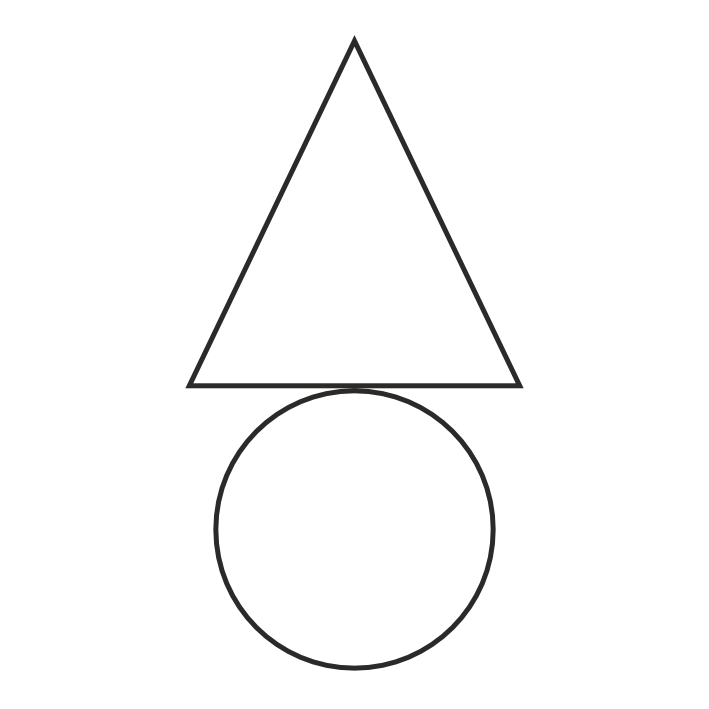
\includegraphics[scale=0.3]{./img/tr}
	\hfill~
\end{minipage}
\begin{minipage}{0.5\linewidth}\setlength{\parindent}{1.5em}
\epigraph{\textit{Раз, два, три, четыре, пять, шесть, семь, восемь, девять, десять -
		можно все пересчитать, или же измерить, взвесить...
}}{Считалка из учебника математики для 1 класса}
\end{minipage}
\end{figure}

\begin{figure}[h!]
\begin{minipage}{0.84\linewidth}\setlength{\parindent}{1.5em}
Пусть у нас есть три треугольника и два круга. Мы хотим составить фигурку такую как на рисунке сверху. Сколькими способами мы можем это сделать? Понятно, что выбор круга и выбор треугольника никак не зависят друг от друга. С любым из кругов можно выбрать любой из треугольников. Возможные комбинации приведены на рисунке справа. Итого 6 вариантов. 
\end{minipage}
\begin{minipage}{0.15\linewidth}
    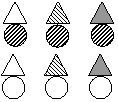
\includegraphics[width=0.9\columnwidth]{./img/tre}
\end{minipage}
\end{figure}

\begin{figure}[h!]
\begin{minipage}{0.15\linewidth}
    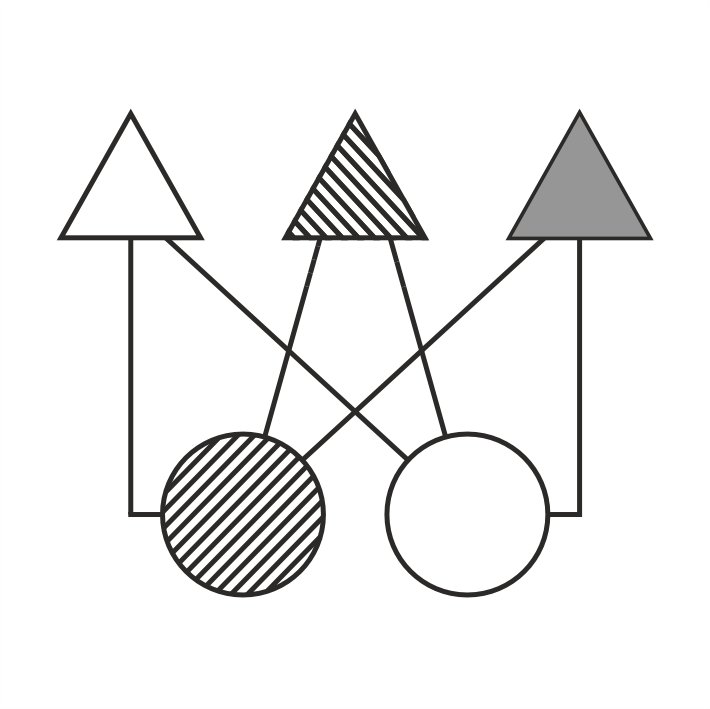
\includegraphics[width=0.9\columnwidth]{./img/komb}
\end{minipage}
\begin{minipage}{0.84\linewidth}\setlength{\parindent}{1.5em}
Этот же факт можно проиллюстрировать по-другому - см. рисунок слева. Те фигурки, которые можно поставить в пару, соединены линией. Сколько линий, столько и вариантов. И наконец третья иллюстрация - треугольник мы можем выбрать тремя способами, а круг - двумя, следовательно, всего $3 \times 2 = 6$ вариантов.\\ Итак, окончательный \underline{\textit{ответ:}} 6 способов.
\end{minipage}
\end{figure}

\begin{figure}[!h]
\begin{minipage}{0.84\linewidth}\setlength{\parindent}{1.5em}
\begin{thm}
	Из города A в город B ведут 3 дороги, а из города B в город C - 2 дороги. Сколькими способами можно проехать из A в C? 
\end{thm}
\begin{prf} Понятно, что выбор дороги между А и В никак не связан с выбором дороги между В и С. Поэтому из А в В мы можем доехать тремя способами, а из В в С - двумя способами. Поэтому всего способов - $3 \times 2 = 6$. \underline{\textit{Ответ:}} 6 способов.\footnotemark
\end{prf}
\end{minipage}
\begin{minipage}{0.15\linewidth}
    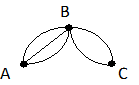
\includegraphics[width=0.9\columnwidth]{./img/ways}
\end{minipage}
\end{figure}
\footnotetext{Заметим, что эта задача полностью аналогична предыдущей задача про выбор треугольников и кружков: можно, например, считать, что дороги из А в В помечены одним из треугольников и выбор дороги означает выбор треугольника, а дороги из В в С помечены кругами и выбор дороги означает выбор одного из двух кругов.}

\begin{figure}[!h]
\begin{minipage}{0.2\linewidth}
    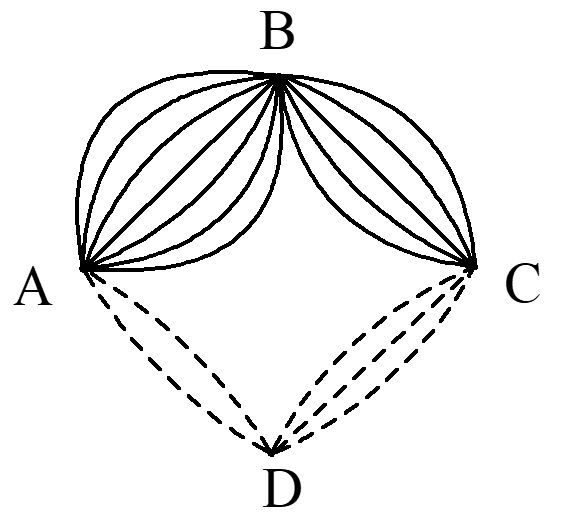
\includegraphics[width=0.9\columnwidth]{./img/ways2}
\end{minipage}
\begin{minipage}{0.79\linewidth}\setlength{\parindent}{1.5em}
\begin{ex}\label{u14}
	а) Из города А в город В ведут 7 дорог, а из города В в город С - 5 дороги. Сколькими способами можно проехать из А в С?
	\\	
	б) Построили новый город D и из него 2 дороги ведут в А и 3 в С. Сколькими способами теперь можно проехать из А в С?
\end{ex}
\end{minipage}
\end{figure}

\begin{ex}\label{u15}
	Кощей Бессмертный, желая сделать Бабе Яге подарок на Новый Год, приобрел кучу метелок трех сортов, ступы 5 сортов и головные платки 7 расцветок. Он хочет каждый Новый Год дарить Яге 1 метлу, 1 ступу и 1 платок, но так, чтобы ни один год наборы подарков не совпадали. На сколько лет ему хватит приобретенных товаров?\footnote{Считайте, что количество приобретенных предметов сколь угодно велико.}
\end{ex}

\fbox{
\begin{minipage}{0.93\linewidth}\centering	
\textbf{Основное правило комбинаторики.}

\textit{Если какое-то действие можно разбить на два, и первое из них можно осуществить $n$ способами, а второе - $m$ способами, то все действие можно осуществить $ m\times n$ способами.}
\end{minipage}
}

\begin{ex}\label{u16}
	Переформулируйте предыдущее упражнение как задачу про дороги. 
\end{ex}

\begin{thm}
	Монету бросают трижды. Сколько различных последовательностей орлов и решек можно получить? 
\end{thm}

\begin{prf}
	Для каждого из трех бросков имеется только два варианта: «орел» или «решка». Результат каждого броска не зависит друг от друга. Поэтому вариантов последовательностей восемь. \footnote{При желании их все можно выписать}\\ \underline{\textit{Ответ:}} 8 последовательностей.
\end{prf}

\begin{ex}\label{u17}
	А если в предыдущей задаче бросать монету сто раз?
\end{ex}

\begin{ex}\label{u18}
	Переформулируйте предыдущую задачу как задачу про дороги. 
\end{ex}

\begin{thm}Назовем число симпатичным, если в его записи встречаются только нечетные цифры. Сколько существует симпатичных пятизначных чисел?
\end{thm}

\begin{prf}
	Если цифры могут быть только нечетные, то вариантов для каждой позиции пять (1, 3, 5, 7 и 9). Выбор каждой цифры независим. Поэтому вариантов $5^5$.\\ \textit{\underline{Ответ:}} Всего $5^5$ симпатичных чисел.
\end{prf}

\begin{thm}
	Сколько всего пятизначных чисел, которые не симпатичные, но и не неинтересные?
\end{thm}

\begin{prf}
	Число симпатичное, если в его записи встречаются только нечетные цифры, число неинтересное, если в его записи присутствуют только четные цифры. Поскольку каждая цифра либо четная, либо нечетная, то число не может быть одновременно симпатичным и неинтересным. Поэтому, если мы из общего количества пятизначных чисел вычтем количество симпатичных и количество неинтересных, то получим искомое.
	Всего пятизначных чисел 90000. Это можно сосчитать двумя способами:\\ 1) всего натуральных чисел от 1 до 99999 (последнее пятизначное число) -- 99999, однако числа от 1 до 9999 (всего 9999 штук) -- не более, чем четырехзначные;\\ 2) в пятизначном числе на первом месте может стоять любя цифра кроме 0, поэтому вариантов -- 9, а на каждом их оставшихся четырех местах -- любая из 10 цифр, поскольку выбор каждой цифры осуществляется независимо, то всего $9\times10^4 = 90000$ вариантов.\\
	Сосчитаем теперь количество симпатичных чисел. Поскольку имеется пять нечетных цифр - $1, 3, 5, 7, 9$ и любая из них может стоять на любом из пяти мест, то всего симпатичных пятизначных чисел $5^5$.
	Неинтересные числа: имеется также пять четных цифр - $0, 2, 4, 6, 8$, но на первом месте может стоять лишь одна из четырех (число не может начинаться с нуля). Поэтому вариантов неинтересных пятизначных чисел $4\times 5^4$.
	Итак, искомое количество равно\\ $ 90000 - 5^5 - 4\times 5^4 = 90000 - 5^4 = 90000 - 9\times625 = 90625 - 6250 = 83275 $
\end{prf}

Во многих комбинаторных задачах для записи результата потребуется понятие \textit{факториала}:

\fbox{
\begin{minipage}{0.93\linewidth}\centering	
\textit{Факториалом натурального числа $N$ называется произведение всех целых чисел от 1 до $N$: $N!=1\times 2\times 3\times 4 \times\dots \times (N-1)\times N$ (читается “эн факториал”)}
\end{minipage}
}

Хотя факториал определен только для натуральных $N$, удобно ввести понятие $0!$ - будем считать его равным единице.

\begin{ex}\label{u19}
	Чему равно а) $19!\times20$;~~  б) $6!\times56$;~~  в) $N!\times(N + 1)$?
\end{ex}

\begin{ex}\label{u20}
	Чему равно а) $\frac{101!}{99!}$;~~  б) $\frac{N!}{(N-1)!}$;  
\end{ex}

\begin{thm}
	Сколькими способами можно расположить а) 11 человек в шеренгу;~~ б) 11 разноцветных бусин по кругу?~~ в) Укажите отличия между пунктами а) и б).  
\end{thm}

В предыдущей задаче рассматривается число способов, которыми можно расставить в шеренгу 11 человек. Такое расположение называется \textit{перестановкой}. Таким образом, в этой задаче ищется число перестановок 11 человек. Число перестановок из $N$ предметов обозначается $P_N$.

\begin{thm}\label{3.6}
	Выведите формулу для $P_N$ .
\end{thm}
\head{Ноябрь}{Листок 1. Комбинаторика.}

\textit{В этот раз задачи листочка каждого уровня  рассчитаны на одно занятие. Другими словами, сдавшие 1 уровень и решающие второй, имеют времени только одно занятие – сегодняшнее. Сдающие также и первый имеют в свoем распоряжении два занятия – это и еще следующее. После чего все задачи обоих уровней будут разобраны.}

\begin{thm}
	Сколько диагоналей и сторон у выпуклого  а) 23-угольника;~~~ б) n-угольника?
\end{thm}

\begin{thm}
	Сколько есть возможностей поставить на шахматную доску\\ а) белую и черную~~~б) две черных ладьи так, чтобы они не били друг друга?~~~в) Укажите отличия между пунктами а) и б).
\end{thm}

\begin{thm}
	Сколько существует шестизначных чисел с разными цифрами?
\end{thm}

\begin{thm}
	У нас есть 13 шариков – 12 черных и 1 зеленый. Найдите число а) всех перестановок; б) всех различных перестановок.\footnote{Одинаковыми считаются те, при которых шары с одинаковым номерами одного цвета.}
\end{thm}

\begin{thm}
	Та же задача, что и предыдущая, но не один зеленый шарик, а два (всего получается 11 черных и 2 зеленых).
\end{thm}

\begin{thm}
	Шася знает 14 дебютов, 11 миттельшпилей и 13 эндшпилей. Сколь разнообразна Шасина игра в шахматы?\footnote{Дебют – начало партии, миттельшпиль – середина, эндшпиль – окончание.}
\end{thm}

\head{Ноябрь}{Листок 1. Комбинаторика. Проверочная работа.}


\begin{thm}	
	Будем считать число неинтересным, если в его записи присутствуют только четные цифры. Сколько всего неинтересных пятизначных чисел?
\end{thm}

\begin{thm}	
	В алфавите племени Мумба–Бумба всего три буквы: Б, У и М. Словом считается любая не пустая последовательность не более чем из четырех букв. Сколько всего слов в языке племени Мумба–Бумба?
\end{thm}

\begin{thm}
	22 лампочки расположены в ряд. Сколькими способами мы можем зажечь две из них?
\end{thm}

\begin{thm}	
	Сколькими способами можно выбрать в племени 7Ю класса из 20 человек а) вождя и его советника; б) двух дозорных?
\end{thm}

\begin{thm}	
	В Доминандии, как и у нас, есть игра в домино, только точек на домино не от 0 до 6, а от 0 до 2011. Сколько всего доминошек в этой игре?
\end{thm}

\begin{thm}	
	Сколько в мире десятизначных чисел, у которых все цифры разные?
\end{thm}

\begin{thm}	
	Чему равно а) $17!\times 18$;  б) $8!\times 90$;  в) $(N - 2)!\times (N - 1)$?
\end{thm}

\begin{thm}\label{3.4}
	Вычислите а) $\frac{2011!}{2010!}$ ;  б) $\frac{(N+1)!}{(N-1)!}$ ; в)  $\frac{(N+1)!-N!}{N}$
\end{thm}

%\begin{prf}
%	в) $\frac{(N+1)!-N!}{N}=\frac{N!\times (N+1)-N!}{N}=\frac{((N+1)-1)N!}{N}=\frac{N\times N!}{N}=N! $
%\end{prf}

\begin{thm}	\label{3.5}
	Может ли число $N!$ оканчиваться а) одной пятеркой;~~ б) одной восьмеркой;~~ в) семью нулями?
\end{thm}

%\begin{prf}
%	а) Если число оканчивается пятеркой, то по признаку делимости на 5 оно должно делиться на 5. Следовательно, если какой-то факториал оканчивается на 5, то среди его множителей должна быть пятерка. Поэтому это не может быть менее, чем $ 5! $. Но $ 5! $ Оканчивается нулем и, соответственно, последняя цифра равна нулю во всех последующих факториалах.\\  б) Из пункта а) следует, что все факториалы больше 5! Не могут быть искомыми, так как не оканчиваются на 8. Поэтом достаточно проверить оставшиеся первые 5 факториалов: $ 0! = 1 $, не подходит; $ 1! = 1 $ – не подходит; $ 2! = 2 $ – не подходит; $ 3! = 6 $ – не подходит; $ 4! = 24 $ – не подходит. Тем самым доказано, что такого быть не может. в) Заметим, что ноль на конце дает произведение 5 и 2. Поскольку в разложении любого факториала пятерок меньше, чем двоек, то количество нулей на конце совпадает с количеством пятерок в разложении. Посмотрим, какие числа могут давать эти пятерки: 5; 10; 15; 20 – по одной пятерке; 25 – две пятерки. Поэтому факториалы от 0! до 24! Имеют на конце не более 4 нолей, а от 25! до 29! – ровно 6. Факториалы от 30! до 34! Имеют ровно 7 нолей, что требовалось выяснить.
%\end{prf}
\hrule
\section{Решение некоторых задач проверочной}

\textbf{Задача \ref{3.4}}
	Вычислите а) $\frac{2011!}{2010!}$ ;  б) $\frac{(N+1)!}{(N-1)!}$ ; в)  $\frac{(N+1)!-N!}{N}$

\begin{prf}
	в) $\frac{(N+1)!-N!}{N}=\frac{N!\times (N+1)-N!}{N}=\frac{((N+1)-1)N!}{N}=\frac{N\times N!}{N}=N! $
\end{prf}

\textbf{Задача \ref{3.5}}
	Может ли число $N!$ оканчиваться а) одной пятеркой;~~ б) одной восьмеркой;~~ в) семью нулями?

\begin{prf}
	а) Если число оканчивается пятеркой, то по признаку делимости на 5 оно должно делиться на 5. Следовательно, если какой-то факториал оканчивается на 5, то среди его множителей должна быть пятерка. Поэтому это не может быть менее, чем $ 5! $. Но $ 5! $ Оканчивается нулем и, соответственно, последняя цифра равна нулю во всех последующих факториалах.\\  б) Из пункта а) следует, что все факториалы больше 5! Не могут быть искомыми, так как не оканчиваются на 8. Поэтом достаточно проверить оставшиеся первые 5 факториалов: $ 0! = 1 $, не подходит; $ 1! = 1 $ – не подходит; $ 2! = 2 $ – не подходит; $ 3! = 6 $ – не подходит; $ 4! = 24 $ – не подходит. Тем самым доказано, что такого быть не может. в) Заметим, что ноль на конце дает произведение 5 и 2. Поскольку в разложении любого факториала пятерок меньше, чем двоек, то количество нулей на конце совпадает с количеством пятерок в разложении. Посмотрим, какие числа могут давать эти пятерки: 5; 10; 15; 20 – по одной пятерке; 25 – две пятерки. Поэтому факториалы от 0! до 24! Имеют на конце не более 4 нолей, а от 25! до 29! – ровно 6. Факториалы от 30! до 34! Имеют ровно 7 нолей, что требовалось выяснить.
\end{prf}
\head{Ноябрь}{Листок 2. Комбинаторика.}
\begin{thm}
	Пусть теперь дано 9 черных и 4 зеленых шарика. Выясните, сколько существует перестановок, при которых первые 3 шарика зеленые?
\end{thm}

\begin{thm}	
	а) Cколько всего существует различных перестановок 13 шариков из предыдущей задачи?~~~ б) А сколькими способами можно выбрать 3 шарика из 13-ти, разложенных в ряд, шариков?~~~в) Укажите отличия между пунктами а) и б).
\end{thm}

\begin{thm}
	Давайте, заменим 10 черных шариков из задачи 3.10 на 10 разноцветных (получится 13 шариков, среди которых 2 зеленых и 11 других цветов). Вопрос: сколько теперь различных перестановок?
\end{thm}

\begin{thm}
	Теперь добавим 3 синих шарика к 13-ти из задачи 3.14 (будет 16 шариков 12-ти цветов). Тот же вопрос: сколько теперь различных перестановок?
\end{thm}

\begin{thm}	
	Возьмем 10 шариков, среди которых 3 зеленых, 2 черных, 2 белых и 3 других различных цветов. Как много разных перестановок в этом случае?
\end{thm}

\begin{thm}	
	Сколько различных слов (не обязательно осмысленных) можно получить, переставляя буквы в слове МАТЕМАТИКА?
\end{thm}

\begin{thm}	
	Есть на свете некто, кого зовут Словак Разнобукевич. Если взять его фамилию, и стереть несколько букв\footnote{Как минимум одну, но не все!}, сколько различных фамилий может получиться?
\end{thm}

\begin{thm}\label{3.17}
	На бумажной полоске написано слово АБВГДЕЙКА. Сколькими способами можно разрезать эту полоску на три слова? \footnote{Не обязательно осмысленных}
\end{thm}

%\begin{prf}
%	Резать полоску можно только между буквами, поэтому по сути дела задача сводится к выбору промежутков между букв, где нужно поставить перегородки. Так как требуется разрезать на три слова, то надо выбрать два промежутка. Букв всего девять, следовательно, промежутков восемь. Таким образом, задача свелась к задаче о том, сколькими способами можно выбрать два предмета из восьми. Первый предмет можно выбрать восьмью способами, а второй уже только семью. Всего $8\times7=56$ способов. Но каждый из способов мы сосчитали дважды (например, выбор предмета №6 и №8 можно осуществить так: выбрать сначала №6, а потом №8, или наоборот – сначала №8, а затем №6). Поэтому мы должны полученный результат разделить на два. Итак, окончательный \textit{\underline{ответ:}} 28 способов.
%\end{prf}

\begin{thm}
	Дана полоска АБВ … ЮЯ. (всего 33 буквы). Сколько способов разрезать эту полоску на 3 слова?\footnote{Смысл слов не важен.}
\end{thm}

\section{Аналогии}

\begin{thm}
	$^n$Сколькими способами можно разложить 17 одинаковых шаров в четыре ящика? (в каждый ящик нужно положить хотя бы один шар)
\end{thm}

\begin{thm}
	Сколькими способами можно представить число 17 в виде 4 натуральных слагаемых, если способы, отличающиеся порядком слагаемых, различны?\footnote{Например: $4+4+4+5$ и $4+5+4+4$ -- разные случаи.}
\end{thm}

\begin{thm}
	Дана шахматная доска $33\times33$, причем левая нижняя клетка черная. Тогда такой вопрос: сколько есть вариантов положить 3 черные шашки на белые поля в самой верней горизонтали доски?
\end{thm}

\begin{thm}
	Гадкий Миша решил испортить всем новый год – он хочет разорвать елочную гирлянду, состоящую из 22 лампочек, на 4 части (в каждой части должна быть хотя бы одна лампочка, иначе Мише будет неинтересно!) А мы хотим узнать, сколькими способами с такой затеей он может испортить праздник?
\end{thm}

\begin{thm}
	Маленькая Шура решила устроить праздник своим родителям. Для этого она выгребла все монеты из свинки-копилки, пошла в магазин, где продавались воздушные шарики, но обнаружила, что ей не хватает денег, чтоб купить весь магазин, а хватает ровно на 4 шарика. И вот проблема: всего шариков 22 и все разных цветов…. Итак, сколько вариантов у Шуры выбрать 4 шарика из 22 шариков на прилавке?
\end{thm}

\begin{ex}
	Найдите все аналогии из вышеприведенных задач.
\end{ex}

\head{Ноябрь}{Листок 2. Комбинаторика. Проверочная работа}
\begin{enumerate}
	\item В 7Ю учится 20 человек. \\
	a.	Сколькими способами их можно выстроить в ряд? \\
	b.	Сколькими способами их можно выстроить в ряд, если Лиза и Катя хотят стоять рядом? \\
	c.	если Лиза хочет стоять правее Кати (не обязательно рядом)?\\
	d.	если Ваня хочет стоять правее Глеба, а Глеб правее Миши?
\item	В 7Ю учится 20 человек. Сколькими способами можно разбить их на две  равные команды\\
	a.	если эти команды называются Фениксы и Сфинксы.\\
	b.	если мы не различаем эти команды?\\
	c.	Если в Сфинксах и Фениксах может быть не равное число участников.
\item	В 7Ю учится 20 человек – 10 мальчиков и 10 девочек.\\
	a.	Сколькими способами они могут разбиться на пары?\\
	b.	если в паре должны быть мальчик и девочка?\\
	c.	В классе 12 парт. Сколькими способами они могут рассесться в классе?\\
	d.	если они должны сидеть по двое?\\
	e.	если они должны сидеть по двое – мальчик с девочкой?
\item	В 7Ю учится 20 человек. Иван Андреевич хочет выставить им четвертные оценки.\\
	a.	Сколькими способами он это может сделать, если он ставит 2, 3, 4 и 5?\\
	b.	если он не хочет ставить 2?\\
	c.	Если он хочет поставить не больше трех двоек?
\end{enumerate}
	 
\head{Ноябрь}{Листок 3. Комбинаторика.}

\begin{thm}
	$^{\ast}$ Сколькими способами можно представить число $n$ в виде нескольких натуральных слагаемых, если а) $n = 3$;~~ б) $n = 33$;~~ в) $n$ - произвольное натуральное число?
\end{thm}

\begin{thm}
	$^{\ast}$ Сколькими способами можно представить
	а) число 11 в виде 3 целых положительных слагаемых?~~~~
	б) число n в виде 3 целых положительных слагаемых?\\
	в$^{\ast\ast}$) число n в виде  $k < n$  целых положительных слагаемых?\footnote{Способы, отличающиеся порядком слагаемых, считаются различными}
\end{thm}

\begin{thm}
	$^{\ast}$ Сколькими способами можно расставить на шахматной доске восемь\\ а) разноцветных~~~  б) черных ладей, чтобы они друг друга не били?
\end{thm}

\begin{thm}
	$^{\ast}$ Докажите формулу: $(n + 1)! - n! = n!\times n$
\end{thm}

\begin{thm}
	$^{\ast}$ Сколькими способами можно поставить на шахматную доску\\ а) белого и черного~~~ б) двух белых королей так, чтобы они не били друг друга?
\end{thm}

\begin{thm}$^{\ast\ast}$
	\textquotedblleft Распался коллектив музыкального ансамбля племени Мумба-Бумба! На седьмом костре состоится формирование нового музыкального ансамбля из 37 аборигенов!\textquotedblright - звучали Мумб-Бумбские новости, переведенные лингвистами на наш язык. Также ученые выяснили, что в племени Мумба-Бумба были аборигены 7 различных расцветок (в каждой деревне жили аборигены своей расцветки, это как разные флаги в разных странах): Белые, Черные, Красные, Желтые, Синие, Зеленые и Серо-буро-малиновые в крапинку (или в горошек, ученые точно не установили). Возникает весьма интересный и высоко научный вопрос: сколько предстояло тогда Мумб-Бумбскому жюри перебрать различных вариантов составления нового ансамбля, если считать, что аборигены одной расцветки все на одно лицо и что\\
	а) в ансамбле должны присутствовать аборигены всех расцветок?\\
	б) допускается отсутствие в ансамбле аборигенов какой-либо расцветки?
\end{thm}

\begin{thm}
	Каких семизначных чисел больше: тех, в записи которых есть семерка или остальных?
\end{thm}

\begin{thm}$^{\ast\ast}$
	Сколькими способами можно разбить 7А класс (25 человек) на две не обязательно равные группы?
\end{thm}

\begin{thm}$^{\ast\ast}$
	В левом нижнем углу шахматной доски стоит ладья. Сколькими способами она может пройти в правый верхний угол, если она может ходить только вверх и вправо?\footnote{Одними и теми же способами считаются те, когда их пути совпадают.}
\end{thm}
\newpage 

\section{Ответы к упражнениям}
\textbf{\ref{u14}.}	а) 35; б) 41.~~ \textbf{\ref{u15}.} на 105 лет.~~ \textbf{\ref{u16}.} Например, так: из города А в город Б ведет 3 дороги, из города Б в город В 5 дорог, а из города В в город Г - 7 дорог. Сколькими способами можно проехать из города А в Г?~~\textbf{ \ref{u17}.} $2^{100}$.~~ \textbf{\ref{u18}.} Между городами А и В, В и С и С и Д по две дороги. Сколькими способами можно проехать из А в Д?~~ \textbf{\ref{u19}.} а) 20!; б) 8!;  в) $(N+1)!$~~  \textbf{\ref{u20}.} а) $ \frac{101!}{99!}=\frac{99!\times 100\times 101}{99!} = 100\times 101 = 10100$; б) $\frac{N!}{(N-1)!} =\frac{(N-1)!\times N}{(N-1)!} = N$.~~ \textbf{Задача \ref{3.6}}  $P_N=N!$
\section{Решения некоторых задач}
\textbf{Задача \ref{3.17}}
	На бумажной полоске написано слово АБВГДЕЙКА. Сколькими способами можно разрезать эту полоску на три слова? \footnote{Не обязательно осмысленных}

\begin{prf}
	Резать полоску можно только между буквами, поэтому по сути дела задача сводится к выбору промежутков между букв, где нужно поставить перегородки. Так как требуется разрезать на три слова, то надо выбрать два промежутка. Букв всего девять, следовательно, промежутков восемь. Таким образом, задача свелась к задаче о том, сколькими способами можно выбрать два предмета из восьми. Первый предмет можно выбрать восемью способами, а второй уже только семью. Всего $8\times7=56$ способов. Но каждый из способов мы сосчитали дважды (например, выбор предмета №6 и №8 можно осуществить так: выбрать сначала №6, а потом №8, или наоборот - сначала №8, а затем №6). Поэтому мы должны полученный результат разделить на два. 
 
 Итак, окончательный ответ: 28 способов.
\end{prf}
\chapter{Теория Чисел}
\head{Ноябрь}{Листок 4. Теория чисел.}

\begin{figure}[H]
\begin{minipage}{0.4\linewidth}
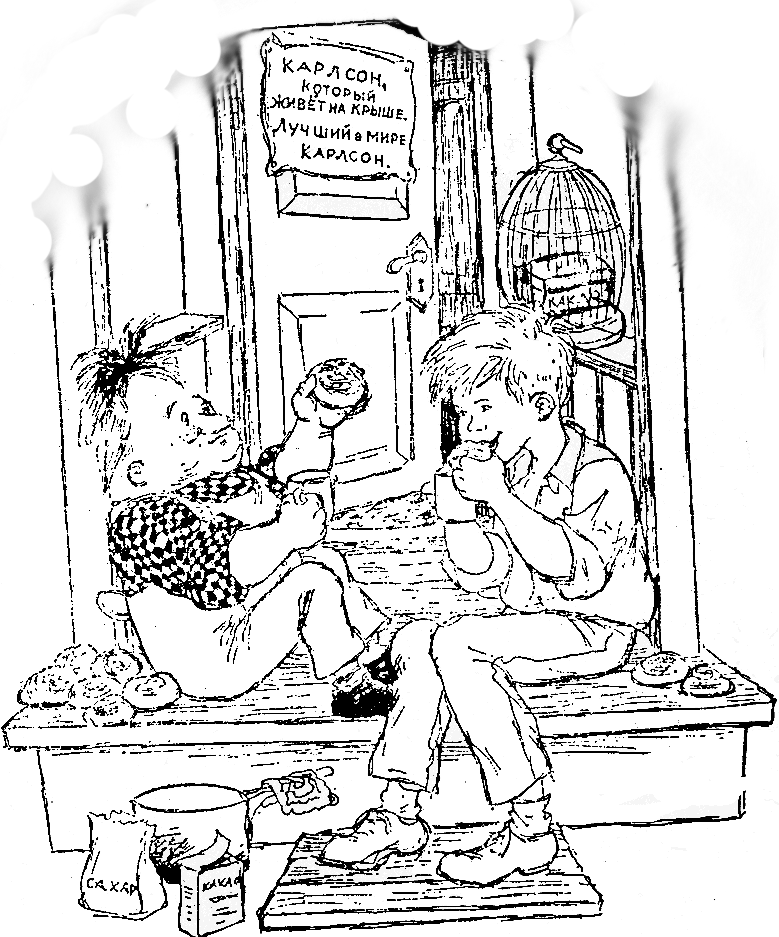
\includegraphics[width=0.9\columnwidth]{./img/karlson}
\end{minipage}
\begin{minipage}{0.55\linewidth}
\epigraph{
\textit{- Мы поделим их поровну: $7$ тебе и $7$ мне, - сказал Карлсон.\\
- Но так не получится, - возразил Малыш. -\\  $7+7=14$, а у нас только $10$ плюшек.\\
- В нынешних школах как-то по-дурацки считают, - ответил тот. - но я из-за этого страдать не намерен. По крайней мере, свои я уже взял, - добавил он и прикрыл пухлой ладошкой дымящуюся горку.
}}{Астрид Линдгрен «Три повести о Малыше и Карлсоне».}
\end{minipage}
\end{figure}

По определению целое число $a$ делится на не равное нулю целое число $b$, если существует целое число $q$ такое, что $a = bq$. В этом случае число $a$ называется делимым, $b$ - делителем, а $q$ - частным. В дальнейшем, речь будет идти только о целых числах.

\fbox{\begin{minipage}{0.95\textwidth}
\begin{ex}\label{u22}
	Запишите общий вид чисел, делящихся а) на 2; б) на 17; в) на 2012.
\end{ex}
\end{minipage}}

\begin{figure}[h]
\begin{minipage}{0.79\linewidth}\setlength{\parindent}{1.5em}
В литературе существует несколько способов обозначить делимость:

Если целое число $a$ делится на целое число $b$, то говорят, что $a$ кратно $b$, пишут $a\del b$. Соответственно запись $a\ndel b$ означает, что $a$ не делится на $b$, или $a$ не кратно $b$. 

Наряду с такими обозначениями используются запись $b~|~a$, означающая, что $a$ делит $b$, т.е. $a$ является делителем $b$. Запись $b~\mathrlap{\backslash}|~a$, что означает, что $a$ не делит $b$, т.е. $a$ не является делителем $b$.
\end{minipage}
\begin{minipage}{0.2\textwidth}
    
\includegraphics[width=0.95\columnwidth]{./img/dog}
\end{minipage}
\end{figure}

Делимость целых чисел обладает несколькими основными свойствами:

\fbox{\begin{minipage}{0.95\textwidth}
\begin{prop}\label{pr1}
Если $a$ и $b$ делятся на $c$, то их сумма и произведение тоже делятся на $c$.
\end{prop}
\end{minipage}}

\begin{dok}
    Поскольку $a\del c$ и $b\del c$, то $a = cq_1$ и $b = cq_2$, где $q_1$ и $q_2$ - целые числа. Следовательно,  $a + b = c(q_1 + q_2)$ и $ab = c_2(q_1q_2)$. Что означает по определению, что $(a + b) \del c$ и $(ab) \del c$, поскольку если    $q_1$ и $q_2$ - целые числа, то их сумма и произведение также являются целыми числами. 
\end{dok}

\fbox{\begin{minipage}{0.95\textwidth}
\begin{prop}\label{pr2}
Если $a\del c$, но $b\ndel c$, то $(ab)\del c$, и $(a + b)\ndel c$.
\end{prop}
\end{minipage}}

\begin{dok}
1) Поскольку $a\del c$, то $a = cq$, где $q$ - целое число. Следовательно, $ab = c(qb)$, т.е. $(ab)\del c$. 2) Доказательство того, что $(a + b)\ndel c$, будем проводить методом «\textit{от противного}». Предположим, что $(a + b)\del c$, тогда из доказанного выше свойства следует, что $(a + b) + (-a)\del c$,\footnote{Здесь одно из слагаемых равно $(a + b)$ , а другое $(-a)$. Вообще говоря, здесь в неявном виде используется утверждение, что «если $a$ делится на $с$, то и $(-a)$ делится на $с$». Докажите это утверждение самостоятельно!} т.е. $b\del c$, но $b \ndel c$ по условию, значит мы пришли к противоречию. Итак, наше предположение, что $(a + b)\del c$, было неверно,  следовательно, $(a + b) \ndel c$.\footnote{При доказательстве теоремы методом «\textit{от противного}» сначала допускают, что утверждение этой теоремы неверно. Затем посредством некоторых рассуждений стараются получить либо заведомо неверное утверждение, либо утверждение, противоречащее условию теоремы. При правильных рассуждениях противоречие может получиться только за счет того, что неверным было первоначальное допущение о том, что теорема неверна. Отсюда делают вывод, утверждение теоремы верно.}
\end{dok}

Пользуясь основными свойствами, решите следующие задачи:

\begin{thm}\label{4.1}
	Докажите, что, если $a\del b$, и $b\del c$, то $a\del c$.
\end{thm}

\begin{thm}\label{4.2}
	Пусть $a \del c$, и $b \del d$. Докажите, что $(ab) \del (cd)$.
\end{thm}

\begin{thm}\label{4.3}
	Даны два числа $a$ и $b$ такие, что $a\del b$. Можно ли утверждать, что $a^n\del b^n$ при любом натуральном $n$?
\end{thm}

\fbox{\begin{minipage}{0.95\textwidth}

\begin{ex}\label{u23}
	Запишите условия предыдущих задач и свойств, используя вместо символа $\del$ символ $|$ .
\end{ex}
\end{minipage}}

\section{Деление с остатком.}

\epigraph{
\textit{Действительность никогда не делится на разум без остатка.
}}{Автор неизвестен}

Отметим на числовой оси точки, соответствующие целым числам. Пусть $b$ - некоторое натуральное (целое положительное) число. Выделим на рисунке все целые числа, кратные $b$. Они расположены на оси на равном расстоянии $b$ друг от друга (Рис. \ref{axis1}). Каждое из этих чисел имеет общий вид $bt$, где $t$ - некоторое целое число. 

\begin{figure}[h]
\begin{subfigure}{.5\textwidth}
  \centering
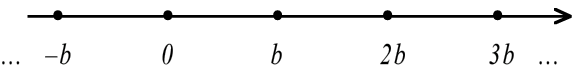
\includegraphics[width=.8\linewidth]{./img/axis1}
  \caption{}
  \label{axis1}
\end{subfigure}%
\begin{subfigure}{.5\textwidth}
  \centering
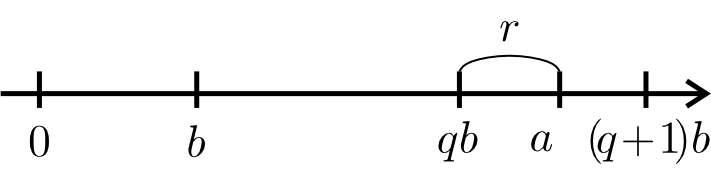
\includegraphics[width=.8\linewidth]{./img/axis2}
  \caption{}
  \label{axis2}
\end{subfigure}
  \caption{}
\end{figure}

Как было определено в начальной школе, если $a = qb$, то $q$ - это частное от деления $a$ на $b$. Будем считать, что остаток в данном случае равен $0$. Попробуем ввести понятие остатка, если целое число $a$ не делится на $b$. Раз $a$ не кратно $b$, то оно попадает между двумя выделенными числами, пусть эти числа $qb$ и $(q+1)b$ (Рис. \ref{axis2}). Тогда число $r = a - qb$ есть целое число, удовлетворяющее неравенству $0 < r < b$. В этом случае назовем частным число $q$, а остатком число $r$. 

Теперь сформулируем общее утверждение:

\fbox{\begin{minipage}{0.95\textwidth}
Если $a$ и $b$ - целые числа, причем $b$ больше нуля, то существуют такие целые числа $q$ и $r$, что $a = bq + r$, где $r$ удовлетворяет неравенству $0  \leqslant r < b$. Эти числа $q$ и $r$ определяются по данным $a$ и $b$ единственным образом. Частным называется число $q$, а остатком число $r$.
\end{minipage}}

Чтобы найти частное $q$ и остаток $r$, не нужно, конечно, рисовать отрезок длины $a$ на числовой оси и «укладывать» на нем много раз отрезок длины $b$. Для этого существует более рациональный способ. Это - известное всем правило деления одного числа a на другое число $b$ «столбиком». Это деление можно производить до тех пор, пока остаток не станет меньше, чем делитель. Например, если делить 1999 на 17, то при делении получается частное 117 и остаток 10.

\begin{prim}
В утверждении, обведенном в рамочку, сказано, что делитель $b$ - положительное число, и остаток таков, что $0  \leqslant r < b$, но делимое $a$ при этом может быть как положительное, так и отрицательное или вообще равное $0$. Например, $a = -22$, $b = 7$, тогда   $(-22) = (-4)\cdot 7 + 6$, где $0 \leqslant 6 <7$, т.е. остаток при делении $(-22)$ на 7 равен 6.
\end{prim}

\fbox{\begin{minipage}{0.95\textwidth}
\begin{ex}\label{u24}
	Какой остаток дает число\\
а) -1 при делении на 7;\hfillб) (-150) при делении на 19;\hfillв) (-54321) при делении на 4?
\end{ex}
\begin{ex}\label{u25}
	Докажите, что числа а) $10^4$ и $10^6$; \hfill    б) $10^5$ и $-1$;    \hfill   в) -123456789 и 9876543210 	\\
дают одинаковые остатки при делении на 11.
\end{ex}
\end{minipage}}

Докажем основные свойства остатков:

\fbox{\begin{minipage}{0.95\textwidth}
\begin{prop}
Если к произвольному целому числу $x$ прибавить число $y$, делящееся на $c$, то остаток при делении $x$ на $c$ не изменится.
\end{prop}
\end{minipage}}

\begin{dok}
Пусть $x = cq + r$, $y  = cs$, тогда $x$ будет равен $c(q + s) + r$, где $0 \leqslant r < c$,\footnote{Объясните, почему это неравенство верно.} т.е. остаток не изменился.
\end{dok}

\fbox{\begin{minipage}{0.95\textwidth}
\begin{prop}
Если при делении на $c$ целые числа $a$ и $b$ дают остатки $r_1$ и $r_2$ соответственно, тогда суммы      $(a + b)$ и $(r_1 + r_2)$ при делении на $c$ дают одинаковые остатки.
\end{prop}
\end{minipage}}

\begin{dok}
Пусть $a = cq_1 + r_1$, $b = cq_2 + r_2$, тогда $(r_1 + r_2) = (a + b) - c(q_1 + q_2)$. Из доказанного выше свойства $0$ следует, что $(a + b)$ и $(r_1 + r_2)$ при делении на $c$ дают одинаковые остатки. 
\end{dok}

\fbox{\begin{minipage}{0.95\textwidth}
\begin{prop}
Если при делении на $c$ целые числа $a$ и $b$ дают остатки $r_1$ и $r_2$, тогда произведения $(ab)$ и $(r_1r_2)$ при делении на $c$ дают одинаковые остатки.
\end{prop}
\end{minipage}}

\begin{dok}
Пусть $a = cq_1 + r_1$, $b = cq_2 + r_2$, тогда $(r_1r_2) = (ab) - c(q_1q_2с + q_1r_2 + r_1q_2)$, т.е. $(ab)$ и $(r_1r_2)$ при делении на $c$ дают одинаковые остатки, т.к. отличаются на число, кратное $c$.
\end{dok}

С помощью этих свойств очень легко находить остатки.\footnote{По существу мы с вами доказали, что если нам интересуют только остатки, то на любом шаге вычислений мы можем рассматривать только остатки, пренебрегая целой частью.}

\begin{samp}
16131 при делении на 13 дает остаток 2. Действительно,   $16131 = 131 + 16\cdot10\cdot10$,    где 131 дает остаток 1,  а у числа $16\cdot10\cdot10$ такой же остаток, как и у числа  $3\cdot(-3)\cdot(-3)$. Остаток у 16131 такой же, как остаток у числа $(1+27)$, значит, он равен 2.
\end{samp}

Рассмотрим все числа, которые дают остаток $r$ при делении на $b$. Чтобы отметить все такие числа на числовой оси, надо взять отмеченные ранее числа, кратные $b$ (Рис. \ref{axis1}), и сдвинуть их вправо на $r$ (Рис. \ref{axis3})

\begin{figure}[h]
  \centering
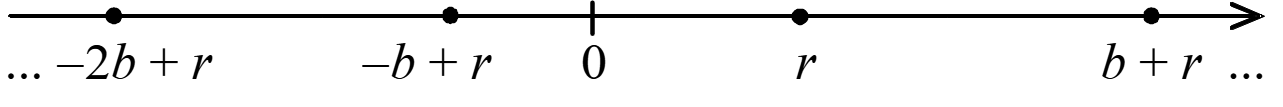
\includegraphics[width=.5\linewidth]{./img/axis3}
  \caption{}
  \label{axis3}
\end{figure}

Отметим, что общий вид числа, дающего остаток $r$ при делении на $b$, это $x = bt + r$,\footnote{Заметим, что в качестве $r$ вовсе не обязательно брать остаток от деления, можно взять любое другое число, дающее тот же остаток. Просто взятие остатка зачастую является наиболее удобным для понимания того, как устроен данный набор чисел.} где $t$ - произвольное целое число. Пусть в этой формуле $t$ пробегает все множество чисел {..., 2, 1, 0, 1, 2,...}, в то время как $b$ и $r$ фиксированы и не меняются (скажем, $b=8$,  $r=5$, тогда $x=8t+5$). При этом формула дает все возможные целые числа, для которых остаток от деления на $b$ равен $r$. Если изобразить эти числа на оси, то получится множество точек, отстоящих друг от друга на расстоянии $b$ (см. Рис. \ref{axis3} и Рис. \ref{axis4} - на последнем приведено множество точек $x=8t+5$).

\begin{figure}[h]
  \centering
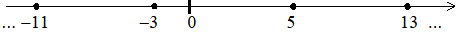
\includegraphics[width=.5\linewidth]{./img/axis4}
  \caption{}
  \label{axis4}
\end{figure}

Таким образом, если задано $b > 0$, то все множество целых чисел можно разбить на $b$ классов: к одному классу отнести все числа, дающие при делении на $b$ остаток 1, к другому - остаток 2, и так далее. Эти классы можно записать так:

\begin{center}
    $x=bt+1$; \hspace{3mm} $x=bt+2$; \hspace{3mm} ...; \hspace{3mm} $x=bt+(b-1)$
\end{center} 

и, наконец, последний (вернее «нулевой») класс $x = bt$. В него входят все числа, дающие при делении на $b$ остаток 0, т.е. делящиеся на $b$. (Например, если $b=8$, то всего классов 8: $x = 8t$, $x = 8t + 1,$ ..., $x = 8t + 7$.) Каждое число обязательно попадает в один и только в один класс. То есть число не может давать двух различных остатков при делении на одно и то же число.\footnote{Это утверждение означает корректность определения деления с остатком.}

ИТАК:

Множество всех чисел $с$ остатком $r$ при делении на $b$ образуют один класс, называемый классом $r$ по модулю $b$ (например, класс 5 по модулю 8 это множество всех чисел, которые дают остаток 5 при делении на 8). Если взять произвольное целое число $x$ и рассмотреть его по модулю $n$, то чтобы определить в каком классе находится наше число, надо рассмотреть его остаток при делении на $n$ (например, $x = 13$, а $n = 8$, тогда число $x$ попадает в класс 5 по модулю 8). Таким образом, если взять натуральное число $n$, то все целые числа разбиваются ровно на $n$ классов, и каждое целое число попадает ровно в один из них.\footnote{Заметим, что множества всех целых чисел, дающих одинаковый остаток при делении на $n$, называют также классами вычетов по модулю $n$. Обозначают $ \tilde{d} = \{ z \in \mathbb{Z} | z - d \del n\}$ - это все числа, имеющие одинаковый с числом $d$ остаток при делении на $n$. Например, числа -1, 3, 7 попадают в класс вычетов $\tilde{3}$ по модулю 4.}

\underline{Обозначение}: A $\equiv$ B (mod C), если А и В дают одинаковые остатки при делении на С.

\fbox{\begin{minipage}{0.95\textwidth}
\begin{ex}\label{u26}
	Запишите общий вид числа, которое при делении а) на 22 дает такой же остаток, что и 2012; б)  на 13 дает такой же остаток, что и 31; в) на 2012 дает такой же остаток, что и (-22).
\end{ex}
\begin{ex}\label{u27}
    Определите, к какому классу относится число а) 2012 по модулю 17; б) 2012 по модулю 2011; в) (-2010) по модулю 22; г) $2004^{13}$ по модулю 1024?
\end{ex}
\begin{ex}\label{u28}
    Выясните, какие из утверждений являются верными: \\
    а) 5 $\equiv$ 17 (mod 2); б) 21 $\equiv$ 154 (mod 5); в) -21 $\equiv$ 154 (mod 5); г) 2007 $\equiv$ 2021 (mod 19); д) 1234567897 $\equiv$ 7987654321 (mod 9); е) 17 $\equiv$ -17 (mod 3).
\end{ex}
\begin{ex}\label{u29}
    Может ли целое число одновременно находиться в классах 1 по модулю 7, 1 по модулю 9, 1 по модулю 11, 1 по модулю 13? (Если да, то приведите пример такого числа, если нет, то докажите, что их нет.) 
\end{ex}
\end{minipage}}

\fbox{\begin{minipage}{0.95\textwidth}
\begin{prop}
Два числа $x_{1}$ и $x_{2}$ попадают в один и тот же класс по модулю $b$ в том и только в том случае, если их разность $x_1 - x_2$ делится на $b$. 
\end{prop}
\end{minipage}}

Выше мы уже говорили, что числа, делящиеся на $n$, расположены на числовой оси «равномерно», то есть через каждые $n$ - 1 чисел. Как каждое второе число является четным (и, соответственно, среди двух последовательных чисел обязательно найдется четное) так и каждое третье число делится на 3 (и, соответственно, среди трех последовательных чисел будет ровно одно, делящееся на три). Эти свойства используются при решении многих задач.

\begin{thm}\label{4.4}
	Докажите, что произведение трех последовательных чисел делится на 6.
\end{thm}

\begin{dok}
    Поскольку среди любых двух последовательных чисел одно обязательно четное, то произведение делится на 2. Кроме того, среди любых трех последовательных чисел одно обязательно делится на 3, значит, произведение делится на 3. Поэтому произведение делится на 6. 
\end{dok}
\begin{floatingfigure}[L]{0\textwidth}
\end{floatingfigure}

\textit{\textbf{Внимание!}} Мы при доказательстве воспользовались тем фактом, что если число (в данном случае произведение трех последовательных чисел) делится на 2 и на 3, то оно делится на 6. Более общий факт: 

\fbox{\begin{minipage}{0.95\textwidth}
\begin{prop} 
Если число А делится на $b$ и делится на $с$ и числа $b$ и $с$ взаимно просты (то есть не имеют общих делителей), то А делится на произведение $bс$. 
\end{prop}
\end{minipage}}

\begin{thm} 
	Докажите, что при любом натуральном $n$ число $n^3 - n$ кратно 6.
\end{thm}

\begin{dok}
    $n^3 - n  =  (n - 1) n (n + 1)$ - произведение трех последовательных чисел. Как было доказано в задаче \ref{4.4}, оно делится на 6.
\end{dok}
\begin{floatingfigure}[L]{0\textwidth}
\end{floatingfigure}

\begin{center}
	{\large\textbf{Десятичная запись числа}}
\end{center}

% \epigraph{\textit{Многие думают, что деньги - это бактерии, которые размножаются делением. Правда, так они думают только о чужих деньгах, а свои деньги просто обязаны размножаться умножением.}}{Из заметок в Интернете}

У чисел, с которыми мы работаем, есть единицы, десятки, сотни… Часто, когда точно неизвестно, каково количество этих самых единиц, десятков, сотен, используют запись с неизвестными: $\overline{xyz}$ - это число, в котором $x$ сотен, $y$ десятков и $z$ единиц, т.е. $\overline{xyz} = 100x + 10y + z$ . В следующих двух  задачах будет полезно представлять числа именно в таком виде. 

\fbox{\begin{minipage}{0.95\textwidth}
\begin{ex}\label{u30}
	Что за числа зашифрованы в записи: а) $\overline{1x}$; б) $\overline{xy5}$; в) $\overline{ab1c0}$ ?
\end{ex}
\begin{ex}\label{u31}
    Пусть некоторое число $a$ делится на простое число $p$. Что вы можете сказать про $a^2$? а про $a^n$?
\end{ex}
\begin{ex}\label{u32}
    Пусть $A$ - квадрат некоторого числа. Выясните, на какую цифру может заканчиваться $A$?
\end{ex}
\begin{ex}\label{u33}
     Известно, что $A$ = $x^2$. При этом $A$ делится на 3. Что вы можете сказать про число $x$?
\end{ex}
\begin{ex}\label{u34}
    Известно, что $A = x^2$. При этом $A$ делится на 2007. Что вы можете сказать про число $x$?
\end{ex}
\end{minipage}}

\newpage

\section{Ответы к упражнениям}
\textbf{\ref{u22}.} а)~$2n$, где $n$ - целое; б)~$17n$, где $n$ - целое; в)~$2012n$, где $n$ - целое. 
\textbf{\ref{u23}.} \textbf{Свойство \ref{pr1}}:~если $c~|~a$  и $c~|~b$, то $c~|~(a~+~b)$ и $c~|~(ab)$; \textbf{Свойство \ref{pr2}}:~если $c~|~a$, но $c~\mathrlap{\backslash}|~b$, то $с~|~ab$, но $c~\mathrlap{\backslash}|~(a+b)$; \textbf{Задача \ref{4.1}}:~докажите, что, если $c~|~b$, а $b~|~a$, то $c~|~a$; \textbf{Задача \ref{4.2}}:~пусть $c~|~a$, а $d~|~b$. Докажите, что $(cd)|(ab)$; \textbf{Задача \ref{4.3}}:~даны два числа $a$ и $b$ такие, что $b~|~a$. Можно ли утверждать, что $bn~|~an$ при любом натуральном $n$? 
\textbf{\ref{u24}.} а)~6; б)~2; в)~3.
\textbf{\ref{u26}.} а)~$22t+2012$ или $22t+10$; б)~$13t+31$ или $13t+5$; в)~$2012t-22$ или $2012t+1990$.
\textbf{\ref{u27}.} а)~$\tilde{6}$; б)~$\tilde{1}$; в)~$\tilde{14}$; г)~$\tilde{0}$.
\textbf{\ref{u28}.} а), в), д).
\textbf{\ref{u30}.} а)~число вида $10+x$, где $x$ - цифра; б)~число вида $100x+10y+5$; в)~число вида $10000a + 1000b + 100 + 10c$.
\textbf{\ref{u31}.} Тогда $a^2$ делится на $p^2$, а $a^n$ делится на $p^n$. 
\textbf{\ref{u32}.} На 0, 1, 4, 5, 6 или 9. 
\textbf{\ref{u33}.} Тогда $x$ также делится на 3.
\textbf{\ref{u34}.} $2007 = 9 \times 223$. Тогда $x$ обязательно делится на $3 \times 223 = 669$.
\head{Ноябрь}{Листок 4. Теория чисел. Уровень 1.}

\begin{thm}
    Докажите, что, если $a \del b$, а $b \del c$, то $a \del c$.
\end{thm}

\begin{thm}
    Пусть $a \del c$, а $b \del d$. Докажите, что $(ab) \skdel (cd)$.
\end{thm}

\begin{thm}
    Даны два числа $a$ и $b$ такие, что $a \del b$. Можно ли утверждать, что $a^n \del b^n$ при любом натуральном $n$?
\end{thm}
    
\begin{thm}
    Известно, что $(ab) \skdel c$ и что $(a+b) \skdel c$. Докажите следующее\footnote{Подсказка: воспользуйтесь формулами сокращённого умножения.}:
    \par 
    а)~$(a^2+b^2) \skdel c$ 
    \par 
    б)~$(a^3+b^3) \skdel c^2$
\end{thm}
    
\begin{thm}
    Докажите, что, если $a^2  \skdel (a + b)$, то и $b^2  \skdel (a + b)$.
\end{thm}

\begin{thm}$^n$ \label{4.1 thm1}
    Докажите, что если $a_1 \del c$, $a_2 \del c$, …, $a_{n-1} \del с$, но $a_n \ndel c$, то $(a_1 + a_2 + ... + a_n)~\ndel c$.
\end{thm}

\begin{thm}
    Глеб на каждой следующей перемене съедает в два раза больше бутербродов с сыром, чем на
предыдущей. Может ли он за две перемены подряд съесть а) 2010 бутербродов? б) 2012?
\end{thm}

\begin{thm}
    В Радужном городе живут 13 чебурашек. У каждого чебурашки есть 3 воздушных шарика:
1 красный, 1 синий и 1 зелёный. Могут ли чебурашки поменяться своими шариками друг с другом так,
чтобы у каждого оказались шарики только какого-либо одного цвета?
\end{thm}

\begin{thm}$^n$ \label{4.1 thm2}
    Группа детского сада построилась парами. Известно, что в каждой паре у одного в три раза больше конфет, чем у второго. Может ли общее число конфет быть равным 2007?
\end{thm}

\begin{thm}
    В одном из подъездов 8-этажного дома на 1 этаже находятся квартиры от № 97 до № 102.
На каком этаже и в каком (по номеру) подъезде находится квартира 178? (на всех этажах одинаковое
число квартир и все подъезды устроены одинаково)
\end{thm}

\begin{thm}
Знайка собирал свои книги в путешествие. Он упаковал все книги в
пачки по 4 штуки. Потом он заметил, что все книги можно упаковать по 6 книг в
каждую пачку. Наблюдавший за всем этим Незнайка воскликнул: «Слушайте, так
ведь если можно упаковать все книги по 4 и по 6 книг в пачку, значит можно
уложить также все книги по 24 в каждой пачке!». Прав ли Незнайка?
\end{thm}

\begin{thm}
    Астроном Стекляшкин тоже задумал упаковать свои книги и отнести на
чердак. Он обнаружил, что если их связывать по 4, по 5 или по 6 книг в пачку, то
каждый раз остается одна лишняя книга, а если по 7 книг в пачку, то лишних книг
не остается. Сколько, самое меньшее, книг хотел отнести на чердак Стекляшкин?
\end{thm}

\begin{thm}
    Прочитав листок «Делимость» и не решив ни одной задачи, Гоша рассердился разорвал его
    на 7 частей. Подумав, он взял некоторые куски и порвал каждый еще на 7 частей, и так далее…. В какой-
    то момент ему это надоело и он ушел в буфет. В это время в класс заглянула Юля и обнаружила 2009
    кусков. Она утверждает, что часть кусков Гоша успел потерять. Можно ли ей верить?
\end{thm}

\begin{thm}
    Лиза решила склеить порванный листок. Она нашла все недостающие кусочки и стала
склеивать всё обратно. Сначала она склеила вместе 4 куска, потом ещё 4 куска, и так
далее… Но, не склеив до конца весь листок, она обнаружила, что ей пора в музыкальную школу. Поэтому она оставила все куски и ушла. Могло ли в результате всех стараний Лизы остаться ровно 2009 кусков?
\end{thm}

\begin{thm}
    Андрей приобрёл в магазине несколько бутылочек лимонада «Black Death» по 35 руб. 77 коп.,
несколько шоколадок по 14 руб. и несколько конфет по 6 руб. 30 коп. за штуку. На кассе ему сообщили, что он должен заплатить 1000 руб. Докажите, что подсчёт произведен неверно.
\end{thm}

\begin{thm}
    Найдите последнюю цифру числа: а) $1999^{1999}$; б) $333^{333}$; в) $2007^{2007}$.
\end{thm}

\begin{thm}$^n$ \label{4.1 thm3}
    Петя купил общую тетрадь объёмом 96 листов и пронумеровал все её страницы по порядку числами от 1 до 192. Вася вырвал из этой тетради 25 листов и сложил все 50 чисел, которые на них написаны. Могло ли у него получиться 2006?
\end{thm}

\textbf{\textit{Внимание! В этот раз в этой части три письменных задачи - \ref{4.1 thm1}, \ref{4.1 thm2} и \ref{4.1 thm3}.}}
\head{Ноябрь}{Листок 4. Теория чисел. Уровень 2.}

\begin{thm}
    Докажите, что число не может попасть в два разных класса (т.е. что число не может давать двух различных остатков при делении на одно и то же число).\footnote{Другими словами мы просим вас доказать корректность определения деления с остатком.}
\end{thm}
    
\begin{thm}
    Можно ли разрезать 6 прутьев длиной по 1 м каждый на 10 кусков длиной 27 см, 16 кусков длиной 15 см и 15 кусков длиной 6 см?
\end{thm}

\begin{thm}
    Докажите, что при любом натуральном $n$ число $n^3 + 3n^2 + 2n$ кратно 6.
\end{thm}

\begin{thm}
    Докажите, что при любом натуральном $n$ число $n(n + 1)^2(3n + 2)$ кратно 4.
\end{thm}

\begin{thm}
    Докажите, что для любого простого $р > 3$ число $р^2 – 1$ делится на 24.
\end{thm}

\begin{thm} $^n$ \label{4.2 thm1}
         Докажите, что при любом натуральном $n$ число $n^3 + 5n$  делится на 3. 
\end{thm}  

\begin{center}
Для решения следующих двух задач рекомендуется вспомнить задачи из листка 2. 
\end{center}

\begin{thm} Докажите, что
    \par 
    а)~из 8 целых чисел всегда можно выбрать два таких, разность которых делится на 7. 
    \par 
    б)~из 5 чисел всегда можно выбрать два таких, у которых разность квадратов делится на 7.
\end{thm}

\begin{thm}
    Докажите, что среди чисел, написанных только единицами найдётся число,
    \\
    делящееся на 2012.
\end{thm}

\begin{thm}
    Докажите, что сумма квадратов двух последовательных целых чисел при делении на 4 даст остаток 1.
\end{thm}

\begin{thm}
    Докажите, что, если число $a^2 + b^2$ делится на 7, то числа $a$ и $b$ делятся на 7.
\end{thm}

\begin{thm} $^n$ \label{4.2 thm2} 
    Число $а$ – чётное, не кратное 4. Докажите, что число $а^2$ при делении на 32 даст остаток 4.
\end{thm}

\begin{thm}
    Число $а$ не делится ни на 2, ни на 3. Найдите остаток от деления числа $а^2$ на 6.
\end{thm}

\fbox{\begin{minipage}{0.95\textwidth}
\begin{thm}
    Докажите, что при любом целом $a$ число $a^2 + 1$ не делится на 3.
\end{thm}
\end{minipage}} 

\begin{center}
Предыдущая задача представляется нам очень важной, поэтому она выделена в тексте \\ и несколько следующих задач используют её же идею. 
\end{center}

\begin{thm}
    Целые числа $х, у, z$ таковы, что $х^2 + у^2 = z^2$. Докажите, что хотя бы одно из этих чисел делится на 3.
\end{thm}

\begin{thm} $^n$ \label{4.2 thm3}
    Может ли сумма квадратов двух целых чисел, не кратных 3, быть квадратом некоторого целого числа?
\end{thm}

\begin{thm}
    Докажите, что остаток от деления натурального числа на 3 (или 9) равен остатку от деления на 3 (или, соответственно, на 9) суммы его цифр.
\end{thm}

\begin{thm}
    Сформулируйте и докажите признаки делимости а)~на 3;~б)~на 9;~в)~на 11.
\end{thm}

\begin{thm}
    Из трёхзначного числа вычли число, получающееся из него же перестановкой цифр. Докажите, что результат вычитания делится на 9.
\end{thm}

\begin{thm} 
     Ваня показывает числовой фокус. Задумайте трёхзначное число с разными цифрами. Запишите его цифры в обратном порядке. Получится ещё одно число. Вычтите из большего числа меньшее. Зачеркните в полученной разности любую цифру, кроме нуля, а оставшееся число сообщите Ване. Ваня тут же назовет вычеркнутую цифру. Как он это делает?
\end{thm}

\begin{thm}
    Найдите все пятизначные числа 
    \par
    а)~вида $\overline{34x5y}$, которые делятся на 36; б)~вида $\overline{71x1y}$, которые делятся на 45. 
\end{thm}

\textbf{\textit{Внимание! На этот раз в этой части три письменных задачи – \ref{4.2 thm1}, \ref{4.2 thm2} и \ref{4.2 thm3}.}}


\head{Ноябрь}{Листок 4. Теория чисел. Уровень 3+.}

\begin{thm}Докажите, что
    \par
    а)~число тогда и только тогда делится на 4, когда две его последние цифры образуют число, \\ делящееся на 4.
    \par
    б)~число тогда и только тогда делится на 8, когда число, составленное из трех последних его цифр делится на 8.
\end{thm}



{
\setlength{\intextsep}{0pt}
\begin{figure}[h]
\begin{minipage}[h]{0.72\linewidth}\setlength{\parindent}{1.5em}
\begin{thm}
    Попробуйте сформулировать и доказать признаки делимости на 7 и на 13.
    \\ 
    {\footnotesize\textit{(\underline{Подсказка}: $1001=7\times11\times13$)}}
\end{thm}
    \begin{thm}
    Перед боем с белогвардейцами у Василия Ивановича и Петьки было поровну патронов. Василий Иванович израсходовал в бою в 8 раз меньше патронов, чем Петька, а осталось у него в 9 раз больше патронов, чем у Петьки. Докажите, что изначально количество патронов у Василия Ивановича делилось на 71. 
    \end{thm}
\end{minipage}
\hfill
\begin{minipage}[h]{0.25\linewidth}
    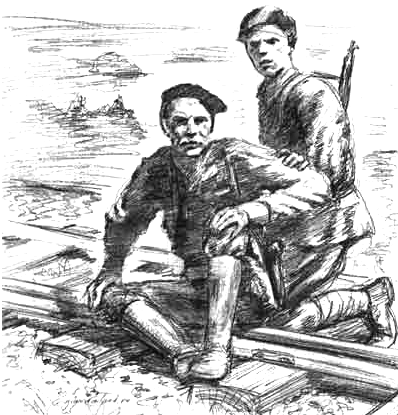
\includegraphics[width=0.9\columnwidth]{./img/soldat}
\end{minipage}

\end{figure}
}

    \begin{thm}
    Автоматический хозрасчётный калькулятор предоставляет следующие услуги:
    \par 
    I)~Умножение имеющегося числа на три за 5 коп.; 
    \par
    II)~Прибавление к имеющемуся числу четырёх за 2 коп. 
    \par
    Число 1 вводится бесплатно. Какую наименьшую сумму нужно потратить, чтобы получить число 2012?
\end{thm}

\begin{thm}$^{\ast}$
Назовём автобусный билет с шестизначным номером счастливым, если сумма цифр его номера делится на 7. Могут ли два билета подряд быть счастливыми?
\end{thm}
{
\setlength{\intextsep}{0pt}
\begin{figure}[h]
\begin{minipage}[h]{0.72\linewidth}\setlength{\parindent}{1.5em}
    \begin{thm}$^{\ast}$
    Шайка разбойников отобрала у купца мешок с монетами. Каждая монета стоит целое число грошей. Оказалось, что какую монету не отложи, оставшиеся монеты можно поделить между разбойниками так, что каждый получит одинаковую сумму. Докажите, что число монет без одной делится на число разбойников в шайке.
    \end{thm}
\end{minipage}
\hfill
\begin{minipage}[h]{0.25\linewidth}
    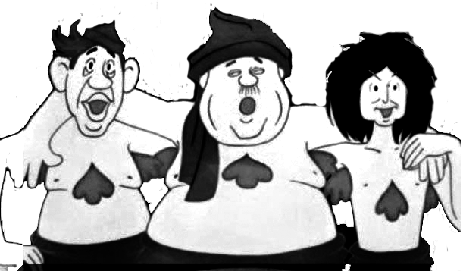
\includegraphics[width=0.9\columnwidth]{./img/razboi}
\end{minipage}
\end{figure}
}
\newpage

\section{Решения некоторых задач.}

\begin{center}
\textbf{Уровень 1.}
\end{center} 

\textbf{Задача \ref{4.1 thm1}.} $^n$
	Докажите, что если $a_1 \del c$, $a_2 \del c$, …, $a_{n-1} \del c$, но $a_n \ndel c$, то $(a_1 + a_2 + ... + a_n) \nskdel c$.
\begin{prf}
    Предположим противное. Т.е. пусть ($a_1+a_2) \skdel c$. Тогда $a_1 + a_2 +$ ... $+ a_n = kc$. В свою очередь $a_i = b_i c$ для всех $i$ от 1 до $n-1$, т.к. по условию $a_i \del c$ для этих значений $i$. Имеем: $a_n = kc - a_1 - a_2 -...- a_{n-1} = kc - b_1 c - b_2 c -$ ... $- b_{n-1}c = c(k - b_1 - b_2 -...- b_{n-1}) = cB$, где $B$ - некоторое целое число, поскольку $k, b_1, b_2,..., b_{n-1}$ по условию целые. 
    Таким образом получаем, что $a_n$ делится на $с$ по определению делимости, что противоречит условию. Следовательно, наше предположение неверно и ($a_1 + a_2 + ... + a_n$) не делится на $c$.
\end{prf}

\textbf{Задача \ref{4.1 thm2}.} $^n$
    Группа детского сада построилась парами. Известно, что в каждой паре у одного в три раза больше конфет, чем у второго. Может ли общее число конфет быть равным 2007?
\begin{prf}
    Рассмотрим общее количество конфет в одной паре. Т.к. у одного из детей конфет в 3 раза больше, чем у другого, то количество конфет у обоих в сумме кратно 4. (если у одного $x$ конфет, то у другого $3x$ конфет и в сумме $4x$) Аналогично кратно 4 количество конфет у любой пары. Поэтому общее количество конфет у всех пар вместе также кратно 4. Но 2007 на 4 не делится. Следовательно, такое суммарное количество конфет быть не может.
\end{prf}

\textbf{Задача \ref{4.1 thm3}.} $^n$
    Петя купил общую тетрадь объёмом 96 листов и пронумеровал все её страницы по порядку числами от 1 до 192. Вася вырвал из этой тетради 25 листов и сложил все 50 чисел, которые на них написаны. Могло ли у него получиться 2006?
\begin{prf}
    Заметим, что нумеруя страницы по порядку, Петя написал на страницах одного листа последовательные числа. Поэтому на любых, в том числе и вырванных, 25-ти листах написаны 25 чётных и 25 нечётных чисел. Сумма таких 50-ти чисел всегда не четна (нечётное число нечётных чисел), поэтому 2006 получиться не могло.
\end{prf}

\begin{center}
\textbf{Уровень 2.}
\end{center}

\textbf{Задача \ref{4.2 thm1}.} $^n$
    Докажите, что при любом натуральном $n$ число $n^3 + 5n$ делится на 3.
\begin{prf}
    \par
    \textbf{\underline{Способ 1}.}
        Рассмотрим 3 случая. 
    \par
        1)~$n$ делится на 3. Но тогда поскольку и $n^3$ и $5n$ делятся в этом случае на 3, то их сумма также делится на 3. 
    \par
        2)~$n = 3k + 1$ ($n$ при делении на 3 даёт остаток 1). Тогда $n^3 = (3k +1)^3 = 27k^3 + 27k^2 + 9k + 1 = 3A + 1$, то есть $n^3$ при делении на 3 также даёт остаток 1. $5n = 5(3k + 1) = 15k + 3 + 2 = 3B + 2$, т.е. $5n$ в этом случае при делении на 3 даёт остаток 2. Отсюда следует, что $n^3 + 5n = 3A + 1 + 3B + 2 = 3(A + B + 1)$ делится на 3. 
    \par
        3)~$n = 3k + 2$ ($n$ при делении на 3 даёт остаток 2). Тогда $n^3 = (3k +2)^3 = 27k^3 + 54k^2 + 36k + 8 = 3A + 2$, то есть $n^3$ при делении на 3 даёт остаток 2. $5n = 5(3k + 2) = 15k + 9 + 1 = 3B + 1$, т.е. $5n$ в этом случае при делении на 3 даёт остаток 1. Отсюда следует, что $n^3 + 5n = 3A + 2 + 3B + 1 = 3(A + B + 1)$ делится на 3. 
    \par
        Поскольку все возможные случаи разобраны, доказательство завершено. 
    \par
    \textbf{\underline{Способ 2}.}
        Скажем, что $n^3 + 5n = n(n^2 + 5)$. Рассмотрим 2 случая.
    \par
        1)~$n$ делится на 3. Тогда и всё выражение делится на 3, т.к. включает в себя множитель, кратный трём.
    \par
        2)~$n$ не делится на 3. Тогда $n^2$ при делении на 3 может давать только остаток 1. \textit{(этот факт был разобран и доказан на уроке и есть в листке - при записи решения доказательство этого факта записывать не нужно)} Тогда $n^2+5$ делится на 3 и всё выражение делится на 3.
    \par
        Поскольку все возможные случаи разобраны, доказательство завершено. 
    \par
\end{prf}

\newpage

\textbf{Задача \ref{4.2 thm2}.} $^n$
    Число $a$ - чётное, не кратное 4. Докажите, что число $a^2$ при делении на 32 даст остаток 4.
\begin{prf}
    $a = 4k + 2$ - такой общий вид у чётных чисел, не кратных 4. Тогда $a^2 = (4k + 2)^2 = 16k^2 + 16k + 4 = 16k(k+1) + 4$. Но $k(k+1)$ - произведение двух последовательных чисел, следовательно, оно чётно. Поэтому $16k(k+1) + 4 = 32A + 4$, где $A$ - целое, что и требовалось доказать.
\end{prf}

\textbf{Задача \ref{4.2 thm3}} $^n$
    Может ли сумма квадратов двух целых чисел, не кратных 3, быть квадратом некоторого целого числа?
\begin{prf}
    Если число не кратно 3, то его квадрат при делении на 3 всегда даёт остаток 1. Тогда сумма двух таких квадратов при делении на 3 даёт остаток 2 и \textit{\underline{не может}} быть полным квадратом, потому что полный квадрат при делении на 3 даёт остаток либо 0, либо 1.
\end{prf}
\chapter{Теория Множеств}
\head{Февраль}{Листок 5. Теория множеств.}
\end{document}